
\documentclass[final,5p,times,twocolumn]{elsarticle}
\usepackage{xeCJK}

\usepackage{mypreamble}
\usepackage{relsize}
\usepackage[inline]{enumitem}
\newcommand\kla[1]{{\textcolor{blue}{Kla: #1}}}
\newcommand\our{OTFCodeGen}
\newcommand\ea[1]{\emph{et al.~}}
\usepackage{tcolorbox}
\newcommand*\circled[1]{\tikz[baseline=(char.base)]{
            \node[shape=circle,draw,inner sep=0.5pt] (char) {\small{#1}};}}
%! Author = sbbfti
%! Date = 10/06/2020
% \newacronym{ts}{$T_{s}$}{supply air temperature, $^{\circ}$C}
% \newacronym{vsp}{$\dot{V}_{sp}$}{volumetric flow rate set-point, L/s}

\newacronym{gtt}{GTT}{Generative Type-Aware Transformers}
\newacronym{mtl}{MTL}{Multi-Tasks Learning}
\newacronym{ifn}{STILTs}{Intermediate Fine-tuning}
% {Supplementary Training on Intermediate Labeled-data Tasks Model}
\newacronym{em}{EM}{Exact Match}
\newacronym{es}{ES}{Edit Similarity}
\newacronym{mrr}{MRR}{Mean Reciprocal Rank}
\newacronym{bpe}{BPE}{Byte Pair Encoding \cite{sennrich2015neural}}
\newacronym{nlp}{NLP}{natural language processing}
\newacronym{ide}{IDEs}{Integrated Development Environments}
\newacronym{ast}{ASTs}{Abstract Syntax Trees}

\begin{document}



   %
% paper title
% Linebreaks \\ can be used within to get better formatting as desired.
% Do not put math or special symbols in the title.
\title{Syntax-Aware On-the-Fly Code Completion}
% \title{Syntax-Aware On-the-Fly Python \\Code Completion with Multi-Task Learning}

\author{Wannita~Takerngsaksiri,~\IEEEmembership{Student Member,~IEEE,}
        Chakkrit Tantithamthavorn,~\IEEEmembership{Member,~IEEE,}
        and~Yuan-Fang Li,~\IEEEmembership{Member,~IEEE.}% <-this % stops a space
\IEEEcompsocitemizethanks{\IEEEcompsocthanksitem W. Takerngsaksiri, C. Tantithamthavorn, Y.-F. Li are with  the Faculty of Information Technology, Monash University, Australia.\protect\\
% \\ is fragile and will error, could use \hfil\break instead.
E-mail: \{wannita.takerngsaksiri, chakkrit, yuanfang.li\}@monash.edu
% \IEEEcompsocthanksitem J. Doe and J. Doe are with Anonymous University.
}% <-this % stops a space
\thanks{Manuscript received November 4, 2022.}}
% revised February XX, 2023.


% The paper headers
\markboth{IEEE Transactions on Software Engineering (TSE),~Vol.~XX, No.~X, November~2022}%
{Wannita \MakeLowercase{\textit{et al.}}: Syntax-Aware On-the-Fly Code Completion}
% \markboth{Journal of \LaTeX\ Class Files,~Vol.~14, No.~8, August~2015}%
% {Shell \MakeLowercase{\textit{et al.}}: Bare Advanced Demo of IEEEtran.cls for IEEE Computer Society Journals}

\IEEEtitleabstractindextext{%
\begin{abstract}

Code completion aims to help improve developers' productivity by suggesting the next code tokens from a given context. 
Various approaches have been proposed to incorporate abstract syntax tree (AST) information for model training, ensuring that code completion is aware of the syntax of the programming languages.
However, existing syntax-aware code completion approaches are not on-the-fly, as we found that for every two-thirds of characters that developers type, AST fails to be extracted because it requires the syntactically correct source code, limiting its practicality in real-world scenarios.
On the other hand, existing on-the-fly code completion does not consider syntactic information yet.
In this paper, we propose \our~to leverage token types, a kind of lightweight syntactic information, which is readily available and align with the natural order of source code.
Our \our~is trained in a multi-task training manner so that by learning the supporting task of predicting token types during the training phase, the models achieve better performance on predicting tokens and lines of code without the need for token types in the inference phase.
Comprehensive experiments show that \our~achieves the first rank on the CodeXGLUE leaderboard with an accuracy of 77.12\% for the token-level predictions, which is 0.43\%-24.25\% more accurate than baselines.
In addition, \our~achieves an exact match of 43.37\% for the line-level predictions, which is 3.63\%-84.73\% more accurate than baselines.
These results lead us to conclude that token type information (an alternative to syntactic information) that is rarely used in the past can greatly improve the performance of code completion approaches, without requiring the syntactically correct source code like AST-based approaches do.
Our \our~is publicly available on HuggingFace.

% Comprehensive experiments show that our model outperforms four state-of-the-art techniques. Specifically, relative to the second-best models, our models achieve an improvement in accuracy of 1.89\% (from 75.69\% to 77.12\%) in token-level prediction and an improvement in an exact match of 8.34\% (from 40.03\% to 43.37\%) in the line-level prediction. 
% On the widely-used CodeXGLUE benchmark, our model sets a new state-of-the-art result.





% A recent study found that code completion can significantly help improve developers' productivity by suggesting the next code tokens from a given context.
% Many current techniques for code completion incorporate abstract syntax tree (AST) information for model training.
% However, we found that , thus limiting the practicality of the AST-based code completion approaches.



% On the other hand, the approaches that require no completeness of source code consider only the sequence of code without syntactic information.


% Code Completion, which helps improve developers' productivity by suggesting the next code tokens from a given context, is one of the most essential features in IDEs. 
% Many current techniques for code completion incorporate abstract syntax tree (AST) information for model training. 
% However, in practice, the AST information requires the syntactically correct and completed source code to be available before it can be extracted. However, AST information may not available for the code completion task at inference time, thus limiting the practicality of these approaches 
% On the other hand, the approaches that require no completeness of source code do not consider syntactic information.
% In this paper, we propose to leverage token types, a kind of lightweight syntactic information, which is readily available even for partially complete code. Our \our: the Syntax-aware On-the-fly code completion model is trained in a multi-task learning manner so that by learning on the auxiliary task of predicting token types, the models achieves better performance on predicting tokens and lines of code.
% Comprehensive experiments show that our model outperforms four state-of-the-art techniques. Specifically, relative to the second best models, our models achieves with an improvement in accuracy of 1.89\% (from 75.69\% to 77.12\%) in token-level prediction and an improvement in exact match of 8.34\% (from 40.03\% to 43.37\%) in line-level prediction. 
% On the widely-used CodeXGLUE benchmark, our model sets a new state-of-the-art result.
% Our models is publicly available at \nolinkurl{HuggingFace}.

% The results indicate that our \our~surpass all baselines achieving the accuracy of 77.12 in token-level prediction and 43.37 in line-level prediction.
% We perform the experiments on both token-level and line-level prediction with various of training techniques. 
% Moreover, we intensively study the impact of the different task weighting parameters and decoding methods.
\end{abstract}

\begin{IEEEkeywords}
Code Completion, Multi-Task Learning
\end{IEEEkeywords}}


% make the title area
\maketitle   

   % Document

\IEEEdisplaynontitleabstractindextext
\IEEEpeerreviewmaketitle
\ifCLASSOPTIONcompsoc
\IEEEraisesectionheading{\section{Introduction}\label{sec:introduction}}
\else
\section{Introduction}
\label{sec:introduction}
\fi

\IEEEPARstart{C}{ode} completion, or AutoCompletion, is one of the most essential features in modern \gls{ide} (e.g., GitHub's Copilot, Intellisense in Visual Studio Code \cite{intelliSense}).
% Tabnine\footnote{https://www.tabnine.com}
The goal of code completion is to automatically recommend source code based on a given context, which could help developers reduce the amount of typing and coding iteration time and eliminate the number of typo errors.
A recent study conducted by Google found that the current code completion feature could reduce developers' effort by 6\% and context switching by 7\%~\cite{ml2022google}.

% the next source code statements given the current context. It can help improve developers productivity by minimize the amount of typing and eliminate typos. These may include pop-up when typing, suggest methods or objects, or query parameters of functions.
% \kla{better to mention the existing tools too, e.g., intellisense, tabnine}\
% \kla{also better to mention the benefit https://ai.googleblog.com/2022/07/ml-enhanced-code-completion-improves.html / check this link and put the reference.}
% Some existing tools are, for example, the code completion in IntelliSense \cite{intelliSense} which is a part of code editing features in Visual Studio Code (VS Code), and Tabnine \footnote{https://www.tabnine.com} which is the AI code assistant for whole-line and full-function code completion that can integrate to many \gls{ide} platforms.

% \kla{2nd para should start from recent work, not the history. this para can be in the related work.}

Recent code completion approaches often leverage modern deep learning architectures (e.g., Recurrent Neural Network, Transformer architecture) to exploit their strong representation power.
More specifically, state-of-the-art code completion models (e.g., CodeGPT~\cite{lu2021codexglue}, GPT-2~\cite{radford2019language}, GPT-C~\cite{svyatkovskiy2020intellicode}, TavTrans~\cite{kim2021code}, CodeFill~\cite{izadi2022codefill}) are based on code-focused large language models (LLMs) that are trained from large codebase and natural language corpora (e.g., the CodeSearchNet corpus with 2 million GitHub repositories). These LLMs are fine-tuned on a specific dataset to perform specific tasks (e.g., code completion).
However, existing code completion approaches have the following limitations.

% For example, Li~\ea~\cite{li2017code} proposed a Pointer Mixture Network model that incorporates the AST information.
% Svyatkovskiy~\ea~\cite{svyatkovskiy2019pythia} proposed Pythia, which is a Long Short-Term Memory (LSTM) network ??? with AST.
% Therefore, researchers proposed to leverage a Transformer architecture, addressing the various limitations of the RNN-based architecture~\cite{kim2021code, liu2020self, izadi2022codefill, liu2022unified}.
% However, such RNN-based and LSTM-based models often suffer from long-term dependencies ???? \kla{what are the limitations of RNN so Transformer is proposed}.


% \kla{bra bra bra , how does it incorporate AST information?}.
% \kla{CodeFill?}


% applying multi-task learning with \gls{ast} \cite{liu2020self}  \cite{izadi2022codefill} \cite{liu2022unified} 
% TravTrans / Transformers+AST  
% GPT-2 (Decoder-only Transformer)
% CodeGPT (Pre-trained Decoder-only Transformer)
% CCAG = flattened \gls{ast} as graphs +  GNN \cite{wang2021code}
% Line-level completion (\cite{wang2020towards}  \cite{izadi2022codefill}
% CodeGPT \cite{lu2021codexglue}
% For code completion in research field, recently it is formulated to an \gls{nlp} task \cite{hindle2016naturalness}. 
% Afterward, many modern NLP techniques has been applied to solve code completion task. For instance, the GPT-style model such as GPT-2 \cite{radford2019language} and language modelling objective have been applied to train with code dataset \cite{lu2021codexglue}. However, some work present that the direct code sequences sometime fail to produce the syntactically correct code \cite{brockschmidt2018generative}, therefore the code language grammar such as \gls{ast} are presented to be utilized to learn the syntactical structures. Many recent works have make use of \gls{ast} for code completion. For instance: 
% . These yield the promising results in code completion.
% using \gls{ast} with LSTM \cite{svyatkovskiy2019pythia},


% From 2012, code completion is migrate \kla{not migrate, but better say 'formulated as an NLP task'? not sure if this is your intention} to \gls{nlp} problem by Hindle et al. \cite{hindle2016naturalness}. Afterward, many NLP techniques has been applied to solve code completion task. There are some works present that the direct code sequences sometime fail to produce the syntactically correct code \cite{brockschmidt2018generative}, therefore the code language grammar such as \gls{ast} are presented to be utilized to learn the syntactical structures. Many recent works have make use of \gls{ast} for code completion \cite{wang2021code} \cite{wang2020towards} \cite{svyatkovskiy2019pythia} \cite{kim2021code} \cite{izadi2022codefill} \cite{liu2020self} \cite{liu2022unified} and yield the promising results.
% \kla{this section needs more details what is each technique and how AST is used?}

\textbf{Limitation 1: \emph{On-the-fly code completions approaches do not consider syntactic information.}}
On-the-fly code completion approaches are designed to generate code tokens based on a given context without requiring the completeness of prior context.
Represent techniques include GPT-2~\cite{radford2019language}, a Transformer-based decoder model for generative tasks pre-trained on English webpage datasets; CodeGPT~\cite{lu2021codexglue}, a GPT-2 model architecture pre-trained on source code datasets; and GPT-C~\cite{svyatkovskiy2020intellicode}, a GPT-2 model architecture pre-trained on multi-language source code. In their pre-training, these models learn to complete the next code tokens. 
In doing so, the performance of these on-the-fly code completion approaches is limited by their lack of consideration of syntactic information.
% provided in the source code.

\textbf{Limitation 2: \emph{Existing syntax-aware code completion approaches are not on-the-fly.}}
To ensure that the generated source code is syntactically correct~\cite{brockschmidt2018generative}, researchers proposed to leverage the Abstract Syntax Tree (AST) information~\cite{li2017code, svyatkovskiy2019pythia, kim2021code, liu2020self, izadi2022codefill, liu2022unified}.
For example, Kim~\ea~\cite{kim2021code} proposed TravTrans, 
% \kla{not clear yet, tell what is this approach}
a Transformer-based architecture consuming syntactic information from a variety representations of ASTs traversal;
Izadi~\ea~\cite{izadi2022codefill} proposed CodeFill, a multi-task,  
% \kla{parallel is a new jargon that is never clearly defined. avoid using it.}
Transformer-based architecture consuming source code and AST types. 
While existing AST-based code completion approaches may generate code that is more syntactically correct, the application scenario remains limited.
In particular, the existing AST-based code completion approaches~\cite{li2017code, svyatkovskiy2019pythia, kim2021code, liu2020self, izadi2022codefill, liu2022unified} require source code to be completed (i.e., all the previous tokens are valid and parsable) at the inference time so the AST information can be obtained from the source code.
However, our motivating analysis found that in practice, two thirds of the source code characters is incomplete and not parsable (e.g., containing syntax errors), making the existing AST-based code completion approaches \emph{inapplicable} in real-world scenarios.
% Second, existing AST-based code completion approaches~\cite{li2017code, kim2021code, izadi2022codefill} are designed to predict an individual code token at the AST node level, not the natural sequence of source code.
% \kla{will mention this later.}



% still focus on the AST node prediction task (i.e., predicting the next AST node based on a given sequence).
% However, such prediction generate the token individually and could not generate the whole line in practical.
% For instance, in Fig.~\ref{fig:motivation} an equivalent source code of an AST node is \textit{logging.getLogger()}, but if we generate the AST node, the \textit{dot} and \textit{parenthesis} characters are not generated. \kla{may be adding an illustrative example figure here. - make a case about on-the-fly....}
% Thus, the AST node prediction can generate only some tokens and not the whole line. 



% However, in real-world scenario, \gls{ast} information is difficult \kla{difficult does not mean possible or impossible} to be correctly retrieve because the syntactically correct and complete source code is hardly present in code completion problems \cite{svyatkovskiy2020intellicode}. \kla{better say what is required to obtain AST information. but in the real-world it may not be available} \kla{it would be great to give an example? ... } Therefore, we propose the use of standard token type information instead of \gls{ast}. The standard token type information can also learn the syntactical data similar to \gls{ast} and more simple to use. It does not require the completeness for parsing and can be retrieve at any points of source code. We present in this work that this information could be useful for code completion.


% However, the evaluation of these papers does not focus on the primary objective of the code completion tasks (i.e., predicting the next code token based on a given sequence of source code).

% However, in real-world scenarios, there are some drawbacks using AST in code completion. Firstly, prediction on \gls{ast} node sequences is not reflect the actual performance of code completion, as it is not the natural order of typing \cite{liu2020multi}. Secondly, AST could create additional overhead and dependencies \cite{svyatkovskiy2020intellicode}. More importantly, last but not least, the syntactically correct and complete source code is hardly present in code completion problems, therefore the ASTs information which required the parse-able code tend to be not available in practical. 

% From the example in Fig. \ref{fig:ASTvsType} and Fig. \ref{fig:ASTfailvsType}. We can observe that the code in Fig. \ref{fig:ASTvsType}a still be able to parse to AST as a result in Fig. \ref{fig:ASTvsType}b. However, with one additional '=' sign in code in Fig. \ref{fig:ASTfailvsType}a, it raises error in AST result in Fig. \ref{fig:ASTfailvsType}b.


\emph{In this paper}, we propose \our, an automated code completion approach that can generate source code at any time regardless of the completeness of the source code, i.e., \textbf{syntax-aware on-the-fly code completion}.
Our approach is designed to consider the syntactic information of the source code during the learning phase, but \emph{does not} require syntactic information during the inference phase.
Instead of using the AST information like in previous works~\cite{kim2021code, izadi2022codefill, li2017code, svyatkovskiy2019pythia, liu2020self, liu2022unified}, we propose to leverage the \emph{token type} information (e.g., String, Number, Name, Keyword), which is a readily-available and light-weight syntactic information without requiring the completeness of the source code.
During the learning process, we design our approach to carry out two prediction tasks, i.e., the token prediction task and the type prediction task.
% Unlike some previous work that leverages AST information as an individual learning objective for the AST node prediction task~\cite{kim2021code,li2017code},
% Our research study on how to best use this token type information along with source code.
To ensure that our model captures both syntactic and semantic information during the training process, we leverage Multi-Task Training (MTT) techniques to learn both the token prediction task and the type prediction task. 
% prediction tasks, and intermediate fine-tuning (STILTs) that sequentially learns from task-to-task.
% To address this challenge of training on multiple tasks (i.e., code prediction and type prediction tasks),
% Particularly, 
Given a sequence of code tokens, our approach performs the following steps: (1) extract the token type information of each token, (2) perform the sub-word tokenization on each token, (3) align token type data with sub-word source code data, and (4) build a code completion model using a GPT-2 architecture based on a pre-trained CodeGPT language model with a multi-task training technique.
% \kla{highlight we don't use the type information at the inference time.}

In our experiment, we compare our \our~with four existing state-of-the-art models (i.e., Pointer Mixture Network~\cite{li2017code}, TravTrans~\cite{kim2021code}, GPT-2~\cite{radford2019language}, and CodeGPT~\cite{lu2021codexglue}).
% \kla{can you add a reference?}).
During the inference phase, we evaluate our approach based on the token-level and line-level prediction tasks.
Through an extensive evaluation on the \textit{PY150}~\cite{raychev2016probabilistic} standard benchmark Python dataset for the code completion task that is used in Microsoft's CodeXGLUE benchmark~\cite{lu2021codexglue}, we answer the following research questions:

% \kla{revised till here}

\begin{description}[leftmargin=1cm, itemsep=3pt]
  \item[RQ1)] \textbf{\rqone}\\
  \textbf{Results.} \fdone

% \our~achieves the first rank on the CodeXGLUE leaderboard with an accuracy of 77.12\% for the token-level predictions, which is 0.43\%-24.25\% more accurate than other baselines.
% In addition, \our~achieves an exact match of 43.37\% for the line-level predictions, which is 3.63\%-84.73\% more accurate than other baselines.

%   Compared with second-best models, \our~achieves an improvement on accuracy of 1.89\% (from 75.69\% to 77.12\%) in token-level prediction and on exact match of 8.34\% %3.34\% 
%   \kla{use relative percentage} 
%   (from 40.03\% to 43.37\%) in line-level prediction.
  
  \item[RQ2)] \textbf{\rqtwo}\\
  \textbf{Results.} \fdtwo

%   the different training techniques can vary accuracy by 2.98\% %2.23\% (from 74.77\% to 77.00\%) in token-level prediction, and 
%   the exact match is different by 11.86\% (i.e., max-min) %4.54\% (from 38.29\% to 42.83\%) in line-level prediction.
  
  \item[RQ3)] \textbf{\rqthree}\\
  \textbf{Results.} \fdthree
%   When adjusting the weights (section~\ref{sec:approach-weight}) of the two tasks (token type prediction and token value prediction), accuracy in token-level prediction can differ by 2.21\% %1.67\% 
%   (from 75.45\% to 77.1\%) and exact match in line-level prediction can differ by 9.05\% %3.6\%
%   (from 39.77\% to 43.37\%).
%   The results show that \our~can perform better in both token-level and line-level predictions when tuning the task weighing parameters.
  
  \item[RQ4)] \textbf{\rqfour}\\
  \textbf{Results.} \fdfour
%   The different decoding methods can vary the results in line-level prediction by 22.84\% %7.72\% 
%   (from 33.80\% to 41.52\%) on exact match and 7.65\% %5.26\%
%   (from 68.72\% to 73.98\%) on edit similarity.
%   Thus, decoding methods have a significant impact on the quality of predictions, and sampling-based methods may not be suitable for the code completion task.
%   Our best suggestion for decoding method as in our setting is Beam search with beam size of 5.
\end{description}


% Therefore inspired by AST, we propose to use standard tokenizer type information. We run the models for python language. The tokens in python are for examples parenthesis, strings, operators, keywords, and variable names. The reasons we use standard tokenizer type information are because: firstly, it maintains the syntactical information similar to \gls{ast}. Second, it is able to retrieve at any points with minimum false representations. Lastly, it is easy to use along the raw source code because it is generated in the similar natural order of typing sequences. The examples compare between AST parser results and standard type results are shown in Fig. \ref{fig:ASTvsType} and Fig. \ref{fig:ASTfailvsType}. We can see that the standard tokenizer type can be retrieved from both source code resulting in Fig. \ref{fig:ASTvsType}c and Fig. \ref{fig:ASTfailvsType}c. Thus, we have this type prediction as the additional non-target task i.e. auxiliary task.

% There are multiple techniques in order to learn the auxiliary task with target task. Nonetheless, in NLP, two essential techniques \cite{weller2022use} are \gls{mtl} and \gls{ifn} \cite{phang2018sentence}. We leverage these techniques and propose TypeComp - the generative type-aware transformers for code completion in this paper. \kla{better highlight what is the challenge of the existing learning technique so multi-task learning is needed}. We intensively train and test models with different training techniques, weighing, and decoding methods in order to find the best architecture of type-aware model for code completion task. Our work is not limit only to a token-level prediction but also include a line-level prediction. We compete TypeComp to 4 state-of-the-arts, additionally we send the results to evaluate on CodeXGLUE Benchmark for code completion task. The results show that TypeComp surpass all state-of-the-art baselines.  



\textbf{Novelty.} The key novelty of our work is as follows:
% \kla{Wannita updates this part too.}
% \kla{TODO later}
\begin{itemize}
    \item \our~is the first to leverage the token type information for code completion with a variety of multi-task training techniques.
    \item \our~is the first to extensively explore the sensitivity of the task weighting parameter and decoding methods in code completion.
    % \item \our~is the first for an empirical study on decoding methods for code completion
    \item \our~surpasses four state-of-the-art code completion techniques and the CodeXGLUE Benchmark, achieving the highest performance in both token-level and line-level predictions.
    \item \our~is publicly available on HuggingFace (\url{https://huggingface.co/Wannita/PyCoder}) together with the token type dataset (\url{https://huggingface.co/datasets/Wannita/PyCoder}).
\end{itemize}

\textbf{Paper Organization.} 
The paper is organized as follows.
Section~\ref{sec:background} describes the background, motivation, and limitations of the state-of-the-art approaches.
Section~\ref{sec:approach} presents our \our~approach. 
Section~\ref{sec:experiment} describes the experimental setup and state-of-the-art baselines. 
Section~\ref{sec:results} presents the experimental results and discussions. 
Section~\ref{sec:discussion} discusses the results of our \our. 
% Section~\ref{sec:relatedwork} presents the related work.
Section~\ref{sec:threats to validity} discloses the threats to validity.
Section~\ref{sec:conclusion} draws the conclusion. 


% The model architectures on \gls{mtl} and \gls{ifn} are explained in session 3. The experimental part is in session 4 which includes dataset (4.1), model training (4.2), post-processing methods (4.3), and baselines information (4.4). The experimental results from 4 research questions are in session 5. Lastly is the discussion and related works in session 6 and 7.

% \begin{figure}
%     \centering
%     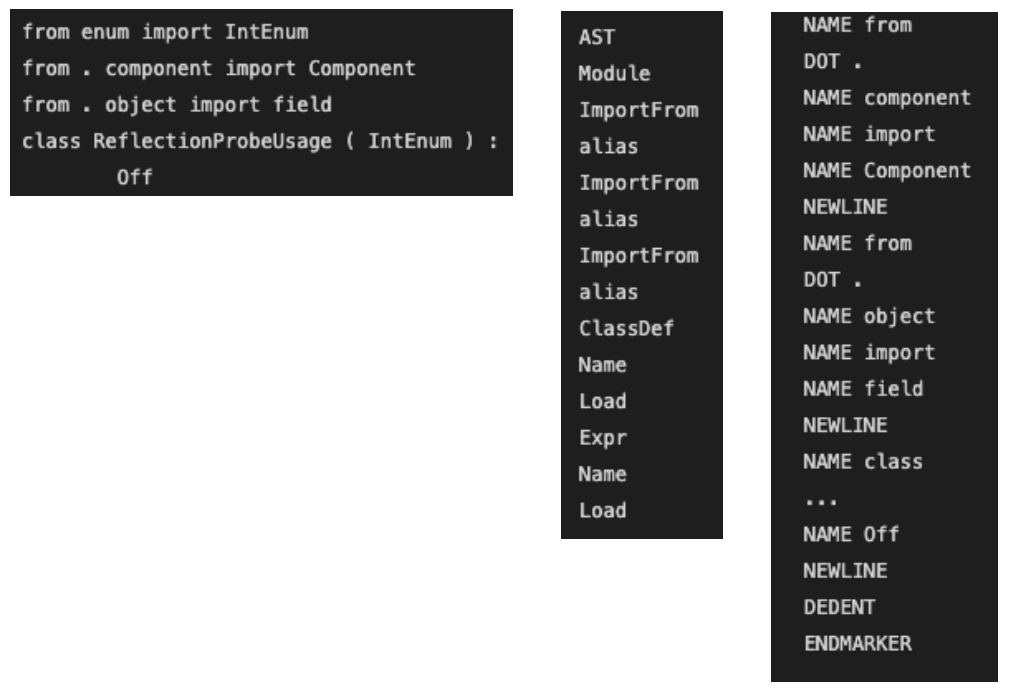
\includegraphics[width=\columnwidth]{figures/motivation2.png}
%     \caption{a) source code example for parsing. b) AST parsing result c) standard token types result}
%     \label{fig:ASTvsType}
% \end{figure}

% \begin{figure}
%     \centering
%     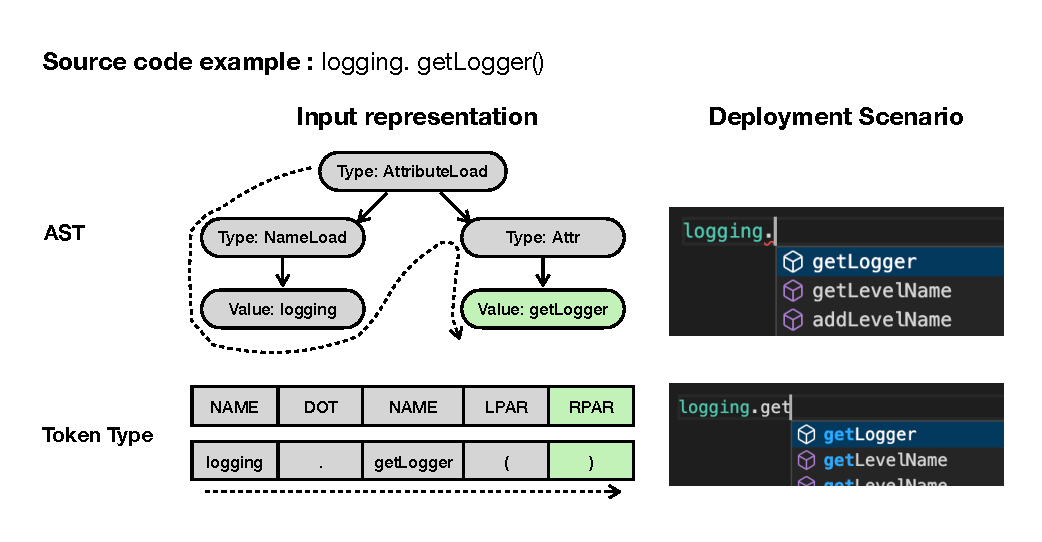
\includegraphics[width=\columnwidth]{figures/motivation.png}
%     \caption{a) source code example for parsing. b) AST parsing result c) standard token types result}
%     \label{fig:ASTfailvsType}
% \end{figure}   
 
    \section{Related Work and Motivation}\label{sec:background} 


In this section, we discuss related work about automated code completion to situate the problems and present a motivating analysis.  

\subsection{Code Completion}
Code completion is a task to suggest the next code token from a given context. More formally, given a sequence of $m$ tokens $x_1 ... x_m$ as a context, code completion aims to predict the next $n$ tokens to complete a sentence $x_1 ... x_{m+n}$. 
The learning objective of a language model for code completion is to minimize a conditional probability distribution of the following function:
% standard language modelling objective that applied to code completion is a conditional probability distribution $P$ as follow:

\[ P(x_{1:m+n}) = \prod_{i=1}^{m+n} P(x_i|x_1 ... x_{i-1}) \]

% There are several approaches proposed for code completion. 
% Starting from the traditional tools by listing out all the possible attributes or methods that can invoke, heuristic rules~\cite{hou2010towards}, program history~\cite{robbes2008program}, and code examples~\cite{bruch2009learning}.

\textbf{Statistical language models.} Previously, several studies proposed code completion approaches using various types of techniques (e.g., heuristic, statistical, and deep learning).
Heuristic-based approaches aim to recommend source code based on rules~\cite{hou2010towards}, program history~\cite{robbes2008program}, and code examples~\cite{bruch2009learning}.
However, heuristic-based approaches are heavily based on rules and patterns that researchers need to develop, which is time-consuming and expensive.
Therefore, statistical language models have been proposed to automatically learn the naturalness of source code based on a probabilistic of the occurrence of source code.
For example, Hindle~\ea~\cite{10.5555/2337223.2337322, hindle2016naturalness} argued that source code is natural and repetitive (similar to natural language) and found that an n-gram approach can accurately predict the next code token based on a given context.
Raychev~\ea~\cite{raychev2016probabilistic} proposed TGEN, a probabilistic-based learning approach with decision tree structures.
However, the statistical language models are able to learn only the limited number of $n$ consecutive tokens (according to the $n$-gram algorithm), which does not reflect the nature of the source code that is usually long (i.e., long-term dependencies).



% Then there are statistical language models to capture the statistical patterns in source code using the occurrence probabilities of sequence of words such as n-gram~\cite{hindle2016naturalness} and decision tree~\cite{raychev2016probabilistic}. 


% Traditionally, code completion is formulated as a probabilistic language model (e.g., n-gram~\cite{hindle2016naturalness}) where the goal is to suggest the next probable code tokens based on a given context of the existing sequence of source code.
% To address various limitations of the traditional probabilistic language models (e.g., \kla{??}), 

% \kla{Gam will do the rest.}
% \kla{need to do this para with Wannita}

% together with the similar characteristic to natural language, code completion is shaped to Natural Language Processing (NLP) problem.
 % in Natural Language Processing (NLP)
 % The model is designed specially to solve the code completion Out-of-Vocabulary (OOV) problem.

\textbf{LSTM-based language models.} To address the limitation of the statistical language models, Long Short-Term Memory (LSTM)-based deep learning approaches are applied to the code completion task.
However, existing LSTM-based language models can only learn the semantic information of the source code, without considering its syntactic structure.
Thus, to ensure that the LSTM-based code completion models recognize the syntactic information, Abstract Syntax Tree (AST) is widely used by the previous work.
For example, Li~\ea~\cite{li2017code} proposed Pointer Mixture Networks, which is an LSTM-based architecture for predicting the AST node. 
Similarly, Svyatkovskiy~\ea~\cite{svyatkovskiy2019pythia} proposed Pythia, which is an LSTM-based approach that incorporates ASTs information through the Word2Vec embedding approach.
While such RNN-based and LSTM-based are able to handle longer sequences of source code than statistical language models, the approach remain inaccurate due to the sequential nature of source code processing, the limited ability to capture long-term dependencies, and the limited ability to recognize the importance of different code tokens.


% Additionally, together with a more complex model, the data such as ASTs information has also been introduced to train the model on syntactical structures of source codes.
% Nonetheless, the early state of deep learning architectures still consider the weight parameters of each token equally which in fact some source code tokens may be less or more important.
% can recognize longer sequences  by recursively inputting the previous output state to the current step. \kla{out of context}
% Next after code completion is shaped to \gls{nlp} problem. There are the coming of deep learning for code completion. The deep neural networks such as RNNs and LSTMs are applied.

\textbf{Transformer-based language models.} 
To address the limitations of LSTM-based language models, the Transformer architecture is introduced for the code completion task.
% Particularly, with the attention mechanism~\cite{vaswani2017attention} inside the Transformer architecture, the model is able to  differentiate the importance of code tokens, allowing the models to pay attention to only the important tokens, not the less important ones.
Generally, the development of Transformer-based language models consists of two steps: pre-training and fine-tuning.
Pre-training is a process to train a Transformer-based language model in a self-supervised manner (i.e., without labels), allowing the language models to self-understand given data by itself (i.e., natural language or programming languages).
Normally, the language models for code completion are trained using a Causal Language Model (CLM) (i.e., predicting the unknown token after a sequence of known tokens).
Once a language model is pre-trained, the model is then fine-tuned on a specific dataset (e.g., PY150~\cite{raychev2016probabilistic}) with the same learning objective as the pre-training process (i.e., CLM).
For example, Lu~\ea~\cite{lu2021codexglue} proposed CodeGPT-based models, which is based on a GPT-2 architecture~\cite{radford2019language} that is pre-trained on both Natural Language (NL) corpus (i.e., WebText) and/or Programming Language (PL) corpus (i.e., CodeSearchNet)---i.e., PL only for CodeGPT, and NL+PL for CodeGPT-adapt.

% from Microsoft Research proposed
To ensure that the Transformer-based language models recognize the syntactic structure of source code, Kim~\ea~proposed TravTrans~\cite{kim2021code}, a vanilla Transformer-based language model that incorporates ASTs information through different encoding styles.
Similarly, Wang~\ea~\cite{wang2021code} leverages AST information with a vanilla Transformer-based language model, but using a different AST encoding technique (i.e., by flattening the ASTs nodes).
However, these AST-based code completion approaches also leverage AST information at the inference phase, which requires source code to be completed at the inference time so the AST information can be parsed and obtained from the source code. 
Therefore, in practice, source code is often incomplete and not compilable (e.g., syntax errors), making the existing AST-based code completion approaches not applicable in real-world scenarios.



% Wang~\ea~\cite{wang2021code}

% the AST information 

% Some work apply flattened ASTs as Graphs then untilize with attention architectures~.


% many representation of ASTs in TravTrans~\cite{kim2021code}, a Transformers-based model to predict AST nodes.


% Not only code sequences but ASTs also still be utilized with Transformers in many works.

% Some work apply flattened ASTs as Graphs then untilize with attention architectures~\cite{wang2021code}.
% Last but not least, currently one of the most powerful generative model is GPT-3~\cite{brown2020language} or Codex~\cite{chen2021evaluating} in software engineering field, however; there are little knowledge on the architecture and training methods in public.




% CodeGPT and CodeGPT-adapt~\cite{lu2021codexglue} are also build up from the same architecture of GPT-2 but are pre-trained on source code dataset (CodeSearchNet).



% variants of the generative pre-train transformers model have been presented, for instance, GPT-2~\cite{radford2019language} is pre-trained from English natural language dataset (WebText) and use to fine-tune on source code.




%and propose SynComp in this work.

% \textit{finish} \kla{end with limitations}


% \subsection{Text Generation Decoding Methods}
% The open-ended text generation is to generate text from the given context. 

% \kla{We may need to provide background: problem/task formulation (token/line)? how code completion is different from other tasks? (the language head?) what is the multi-task learning?}

\begin{figure}[h]
    \centering
    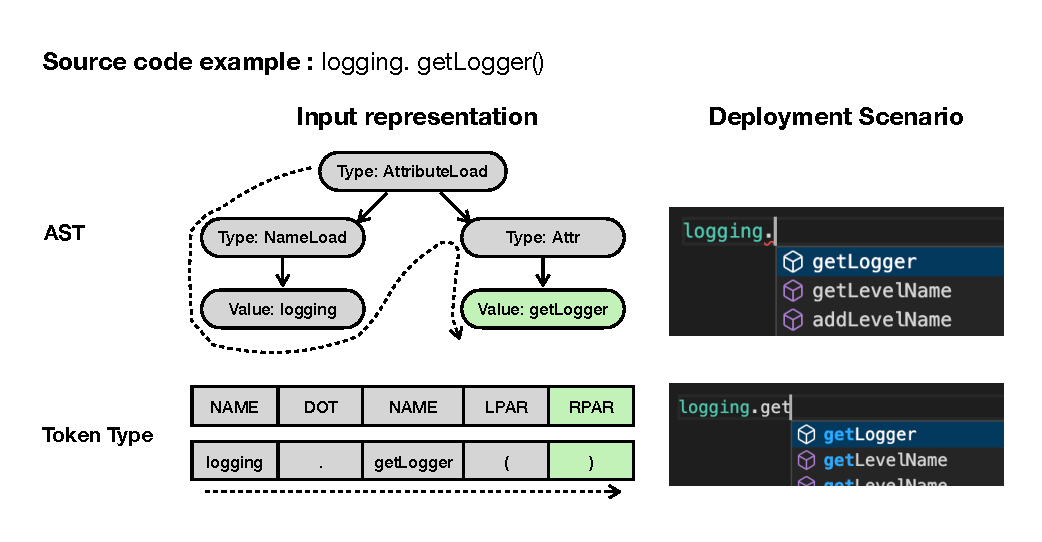
\includegraphics[width=\columnwidth]{figures/motivation.pdf}
    \caption{The comparison between AST and Token Type representations and the ideal deployment scenarios.}
    \label{fig:motivation}
\end{figure}

\subsection{A Motivating Example}

% In this section, we illustrate the limitation of an AST-based code completion approach through a motivating example followed by a motivating analysis.


% \kla{explain the analysis / parsable here / and present the findings. along with Figure 1 and new Figure on the results?}

% In this section, we conduct the analysis to prove the statement that ASTs information is not \emph{on-the-fly} information, i.e. in real-world scenario of code completion task, ASTs information is likely to be unable to extract which lead to the unseemliness of automate code completion.

% In this section, we explain our motivation of this paper.
% There are 2 main motivations: the AST node representation is not a natural order for code prediction, and the AST extraction require the complete and syntactically correct source code as inputs.
% Firstly, 

% \textbf{A Motivating Example.} 
Let's consider a code snippet \texttt{logging.getLogger()} as an example (see Figure~\ref{fig:motivation}).
\texttt{logging.} is the input code token, while \texttt{getLogger()} is the code token to be predicted.
Below, we illustrate two key limitations of the AST-based code completion approach by using TravTrans~\cite{kim2021code} as an example, which makes the existing AST-based code completion \emph{not able to predict next code tokens on-the-fly}.

\emph{First,} the learning objective of TravTrans does not reflect the natural order of typing source code sequences.
Since representing the source code as AST node sequence by traversing the AST, the order of the node sequence are inconsistent with the token sequence~\cite{liu2022unified}.
For example, at the learning phase, TravTrans~\cite{kim2021code} represents the input code tokens as a sequence of an AST node structurekl (i.e., [\texttt{AttributeLoad}, \texttt{NameLoad}, \texttt{logging}, \texttt{Attr}]) in order to predict the next AST node (i.e., [\texttt{getLogger}]).
However, this learning objective does not mimic the natural sequence of code tokens (i.e., [\texttt{logging}, \texttt{.}, \texttt{getLogger}, \texttt{(}, \texttt{)}]), meaning that the programming language-specific characters (e.g., dot [\texttt{.}] and parenthesis [\texttt{(},~\texttt{)}]) are currently ignored.
Therefore, in many cases at the deployment scenarios, such AST node information needs to be post-processed in order to successfully perform code completion in practice (e.g., add missing tokens [\texttt{(},~\texttt{)}], convert [\texttt{Attr}] to [\texttt{.}]).

% With this learning objective, TravTrans requires AST information to be available in order to perform a code completion task.
% This manual post-processing step is also required for other AST-based code completion approaches (e.g., CodeFill by Izadi~\ea~\cite{izadi2022codefill}).
% Unfortunately, this post-processing step remains manual.

% These require the developers' effort to type the missing tokens and/or special post-processing process to convert the nodes back to the source code.
% For example, let's consider the input code token \texttt{logging.} in Figure~\ref{fig:motivation}, TravTrans~\cite{kim2021code} will leverage the \texttt{ast.parse} function provided by the Python AST library to generate the AST node structure for the given input token (i.e., the grey nodes)
% Like in this example, \texttt{logging.} is considered as an AttributeLoad, which consists of two parts, i.e., NameLoad and Attribute.


% The input representation in Fig.~\ref{fig:motivation} shows an example of AST information in TravTrans~\cite{kim2021code} which is represented in node structure.
% TravTrans predicts codes by traversal via AST node in depth-first-search order.
% This kind of node structure is abstract and not the natural order of source code comparing to the code that developers type.

% predicting a sequence of AST nodes (i.e., given a sequence of [AttributeLoad, NameLoad, logging, Attr], then predicting [getLogger])---which does not reflect the natural order of the code sequences that a code completion approach should predict (i.e., given a sequence of [logging.], then predicting [getLogger()]).


% realistic.....

% More specifically, the AST representation in the example has no \emph{dot} and \emph{parenthesis} ( \emph{.} , \emph{(} , \emph{)} ) characters, but \emph{NameLoad} and \emph{Attr} nodes instead.



% These require the developers' effort to type the missing tokens and/or special post-processing process to convert the nodes back to the source code.


\emph{Second,} in order to use AST information as an input, TravTrans~\cite{kim2021code} requires source code to be completed at the inference time so the AST information can be parsed and obtained from the source code. 
For example, in Figure~\ref{fig:motivation}, if developers type \texttt{logging.}, TravTrans can successfully recommend the next token (e.g., \texttt{getLogger)}).
However, source code is often incomplete and not compilable.
For example, in Figure~\ref{fig:motivation}, if developers type \texttt{logging.get}, TravTrans cannot correctly recommend the next token, due to the syntax errors during the AST parsing step.


\subsection{A Motivating Analysis}
\label{sec:motivation}

% \textbf{Motivating Analysis.} 
To demonstrate the significance of the problem of the AST-based code completion approaches, we perform a motivating analysis to investigate how often AST information could be provided at the inference phase, making AST-based code completion can be executed at the inference phase.

% \textbf{Approach.} 
Let's assume that a developer is typing a Python program character-by-character, we aim to analyze how often an AST parser can/cannot successfully parse a Python program at each character.
To do so, we select a statistical representative sample of 383 syntactically correct Python files from the PY150 dataset (with a confidence level of 95\% and a confidence interval of 5\%).\footnote{https://www.surveysystem.com/sscalc.htm}
Since we simulate the application of AST-based code completion at the character level, we execute a Python AST parser\footnote{https://docs.python.org/3/library/ast.html} at each character incrementally.
In total, we execute a Python AST parser for 1,263,296 times according to the total of 1,263,296 characters.
We find that 33.96\% of the executions can be successfully parsed, while 66.04\% of the executions fail to parse due to syntax errors.



\begin{table}[h]
    \centering
    \begin{tabular}{c|c}
        AST Parsable? & Percentage \\
        \hline
        Successful executions & 33.96\% \\
        Failed executions & 66.04\%
        % Success & 28.68\% \\
        % Syntax Error & 71.32\%
    \end{tabular}
    \caption{The percentage of the successful/failed executions of the Python AST parser from the 1,263,296 executions.}
    \label{tab:simulation}
\end{table}

\begin{tcolorbox}
\emph{\textbf{Finding:} For every two out of three characters that developers type, AST-based code completion cannot be performed at all due to the failed execution of the Python AST parser, limiting its ability to perform code completion on-the-fly at the inference time.
Since existing syntax-aware code completion is not on-the-fly and existing on-the-fly code completion is not syntax-aware, this paper aims to address these significant gaps by proposing a syntactic-aware on-the-fly Python code completion approach.
}
\end{tcolorbox}

% While existing syntax-aware 
% }This finding highlights the need for syntactic-aware on-the-fly code completion---that is not yet available.





% Then, we incrementally add one character at a time and parse each time step to AST parser~\footnote{https://docs.python.org/3/library/ast.html}.
% As a result, we receive 1,263,296  typing-simulation timesteps in total.



% we attempt to simulate the real-world scenario that developers are typing the source code character-by-character and count the total results of the successful AST extraction.
% This shows how does AST extracting process perform for the inputs during code completion.



% Moreover, we conduct an analysis to study the AST parsing rate in practice.
% In other word, we attempt to simulate the real-world scenario that developers are typing the source code character-by-character and count the total results of the successful AST extraction.
% This shows how does AST extracting process perform for the inputs during code completion.

% \textbf{Approach.} To simulate the use-case of code completion in practice, we first randomly select 383 python files from PY150 dataset (section 4.1).
% These sample size should allow us to generalize the conclusion about the ratio of ASTs parsing rate to all files with a confidence level of 95\% and a confidence interval of 5\%\footnote{https://www.surveysystem.com/sscalc.htm}.
% Next, normally in coding process (i.e. code completion scenario) the developers type the code character by character.
% Next, to simulate the typing pattern, we split these files into a character-level.
% The special characters (e.g. $\langle EOL \rangle$) are treated as one character.
% Then, we incrementally add one character at a time and parse each time step to AST parser~\footnote{https://docs.python.org/3/library/ast.html}.
% As a result, we receive 1,263,296  typing-simulation timesteps in total.
% Then, we create the typing pattern dataset by sequentially add one character at a time to a new data point.
% As a result, we receive 1,542,810 typing-simulation data points in total.
% Then we parse all data points to ASTs parser using python AST library~\footnote{https://docs.python.org/3/library/ast.html} to find the AST parsing rate for \emph{on-the-fly} scenario.



% \textbf{Results.} \textbf{The AST parser can successfully parse AST }
% Table~\ref{tab:simulation} presents the statistics of the AST parsing rate.
% We find that 




% The result is shown in Table.~\ref{tab:simulation}.
% The number of AST parsing success and error samples are 428,973 and 834,323 respectively, which are represented as 33.96\% and 66.04\% of total samples.
% The number of AST parsing success and error samples are 442,417 and 1,100,393 respectively, which are represented as 28.68\% and 71.32\% of total samples.

% From the simulation results, we can observe that surprisingly most of the time the AST information cannot be extracted.
% More concretely, almost seven out of every ten characters that developers type will fail the AST parsing.
% Not to mention that this is in case of syntactically correct typing only, because our files are from PY150 dataset which has only the syntactically correct files.
% That means in actual cases the successful result of AST parsing rate could be worse than these numbers.

% Therefore, the analysis shows that AST information is not \emph{on-the-fly} information, leading to the limitations of previous works which apply AST information as inputs.
% The example of deployment scenarios in Fig.~\ref{fig:motivation} shows that unlike our token type approach, the AST code completion can only suggest on some positions.
% Such approaches may cause the unseemliness of automate code completion.
% % This also confirms the previous works' limitations, i.e. current code completion approach are either on-the-fly or syntactic-aware but not both.
% % We are motivated by these limitations and propose 
% These findings motivate us and highlights the need for Syntactic-Aware On-the-Fly Code Completion.

   

   \section{Syntax-Aware On-the-Fly Code Completion}\label{sec:approach}


In this section, we present an overview of our syntax-aware on-the-fly Python code completion approach (\our).

Conceptually, \our~aims to generate source code at any time regardless of the completeness of the source code, while considering the syntactic and semantic information of the source code during the learning phase, but \emph{do not} require syntactic information during the inference phase.
To ensure that the learning process considers both semantic and syntactic information, we design our approach to focus on two prediction tasks, i.e., the code token prediction task and the token type prediction task.
In particular, we leverage a Multi-Task Training technique (MTT) to cooperatively learn both the code token prediction task (Task 1: Predict the next code token, considered as a Target Task) and the token type prediction task (Task 2: Predict its token type, considered as a Supporting Task).
For the type prediction task, we propose to leverage the standard Python token type information (e.g., String, Number, Name, Keyword), which is readily available and lightweight, instead of using the AST information~\cite{kim2021code, izadi2022codefill, li2017code, svyatkovskiy2019pythia, liu2020self, liu2022unified} where we found not available for the two-third of the executions (see our finding in Section~\ref{sec:motivation}), limiting its ability to perform on-the-fly code completion.
In contrast, our \our~\emph{does not} require syntactic information at the inference phase.
Thus, the completeness of the source code at the inference time is not required.


% , 
% we found 


% Unlike some previous work that leverages AST information as an individual learning objective for the AST node prediction task~\cite{kim2021code,li2017code},
% Our research study on how to best use this token type information along with source code.
% To ensure that our model captures both syntactic and semantic information during the learning process, we leverage Multi-Task Learning (MTL) techniques to simultaneously learn both the token prediction task and the type prediction task. 



% \textit{Finish}  \kla{please add some key general principles. what is the model? how does the model work? what is the learning objective of the model? how does this model differ from others? why new data collection is needed? what existing dataset is not enough to be used? so we need to perform the following three steps}

% In this section, we present an overview of our approach, \emph{SynComp}, a multi-task training model which learns semantic and syntactic information cooperatively.
% % which learn semantics information via source code, and light-weight syntactic information via token types.
% \kla{should we talk about two prediction tasks somewhere? Task1=? and Task2=}
% The model learn a semantic information from source code which does not require the completeness (i.e. on-the-fly); 
% and apply a token type information to solve the limitation (section 2.2) and learn a light-weight syntactic information (i.e. syntactic-aware).
% Thus, SynComp training phase consists of 2 tasks: source code prediction (target task) and token type prediction (supporting task).
% In order to train the model to learn on multiple task simultaneously, 
% The supporting task (a.k.a. an auxiliary task) is a non-target task that help improve the performance of the target task.
% There are variety techniques on training multi-task SynComp leverage Multi-Task Learning (MTL) and Intermediate Fine-tuning (STILTs) techniques in this work.
% Such techniques have different way

% SynComp leverages Byte-Pair-Encoding (BPE) method~\cite{sennrich2015neural} to handle new unseen tokens; leverages MTL and STILTs~\cite{weller2022use} to address multiple tasks training challenge; and explores varieties of task weighing parameters and decoding methods to find the best perform architecture for code completion.

% In this section, we present an overview of our approach, \emph{SynComp}, a Syntactic-Aware On-the-Fly Code Completion model that learn to complete code with the knowledge enhancement in syntactic information by token types.
% Pure source code sequential model (e.g. CodeGPT and GPT-2) learn semantics data from source code. 
% However, with the support of auxiliary task, i.e. the non-target task which help improve the performance of primary task, such as token type information, SynComp picks up both semantics and syntactic information. 

\textbf{Overview.} Figure~\ref{fig:overview} presents the overview of our \our, which consists of two phases: training and inference.
During the training phase, \our~performs 6 main steps:
Step~\circled{1} Type Extraction, to extract the token type information from source code;
Step~\circled{2} Tokenization, to perform subword tokenization on the source code;
Step~\circled{3} Data Alignment, to align the type information which is word level to the code information which is currently subword level;
Step~\circled{4} Multi-task Training Architecture with 3 training techniques: hard parameters sharing (MTL), soft parameters sharing (MTL), and intermediate fine-tuning (IFN);
then in Step~\circled{5} Hyperparameter Task Weighing and Step~\circled{6} Decoding Methods are the exploration steps to maximize the performance.
For the inference phase, we describe in Step~\circled{7} Code Generation step in the details of token-level prediction and line-level prediction.
% Below, we present the details of each step.

% \textbf{Problem Formulation.} 
% We perform the experiments on 2 kinds of completion level: token-level prediction and line-level prediction.

% MTL - Hard/Soft
% IFT - STILTs

% First, in \emph{(3.1) Data Collection} we extract the token type information from the source code. Then, in \emph{(3.2) Data Processing}, we tokenize the source code with \gls{bpe} algorithm and align the type information to the sub-words. Thus, the training phase consist of 2 tasks: source code prediction and token type prediction. In \emph{(3.3) Model Architectures}, we proposed 3 training techniques: hard parameters sharing MTL, soft parameters sharing MTL, and intermediate fine-tuning. For the inference phase, the model predict the task separately requiring no additional data for each task. Following is the details of our approach.

% We describe our approach in this session. Firstly, we elaborate how we collect the type dataset. Then since our model use BPE tokenizer, we align the type dataset to our source code to be in the same sequences. Lastly, we describe the models experiments which consist of 3 kinds: hard parameters sharing model, soft parameters sharing model, and intermediate fine-tuning model.

\begin{figure*}
    \centering
    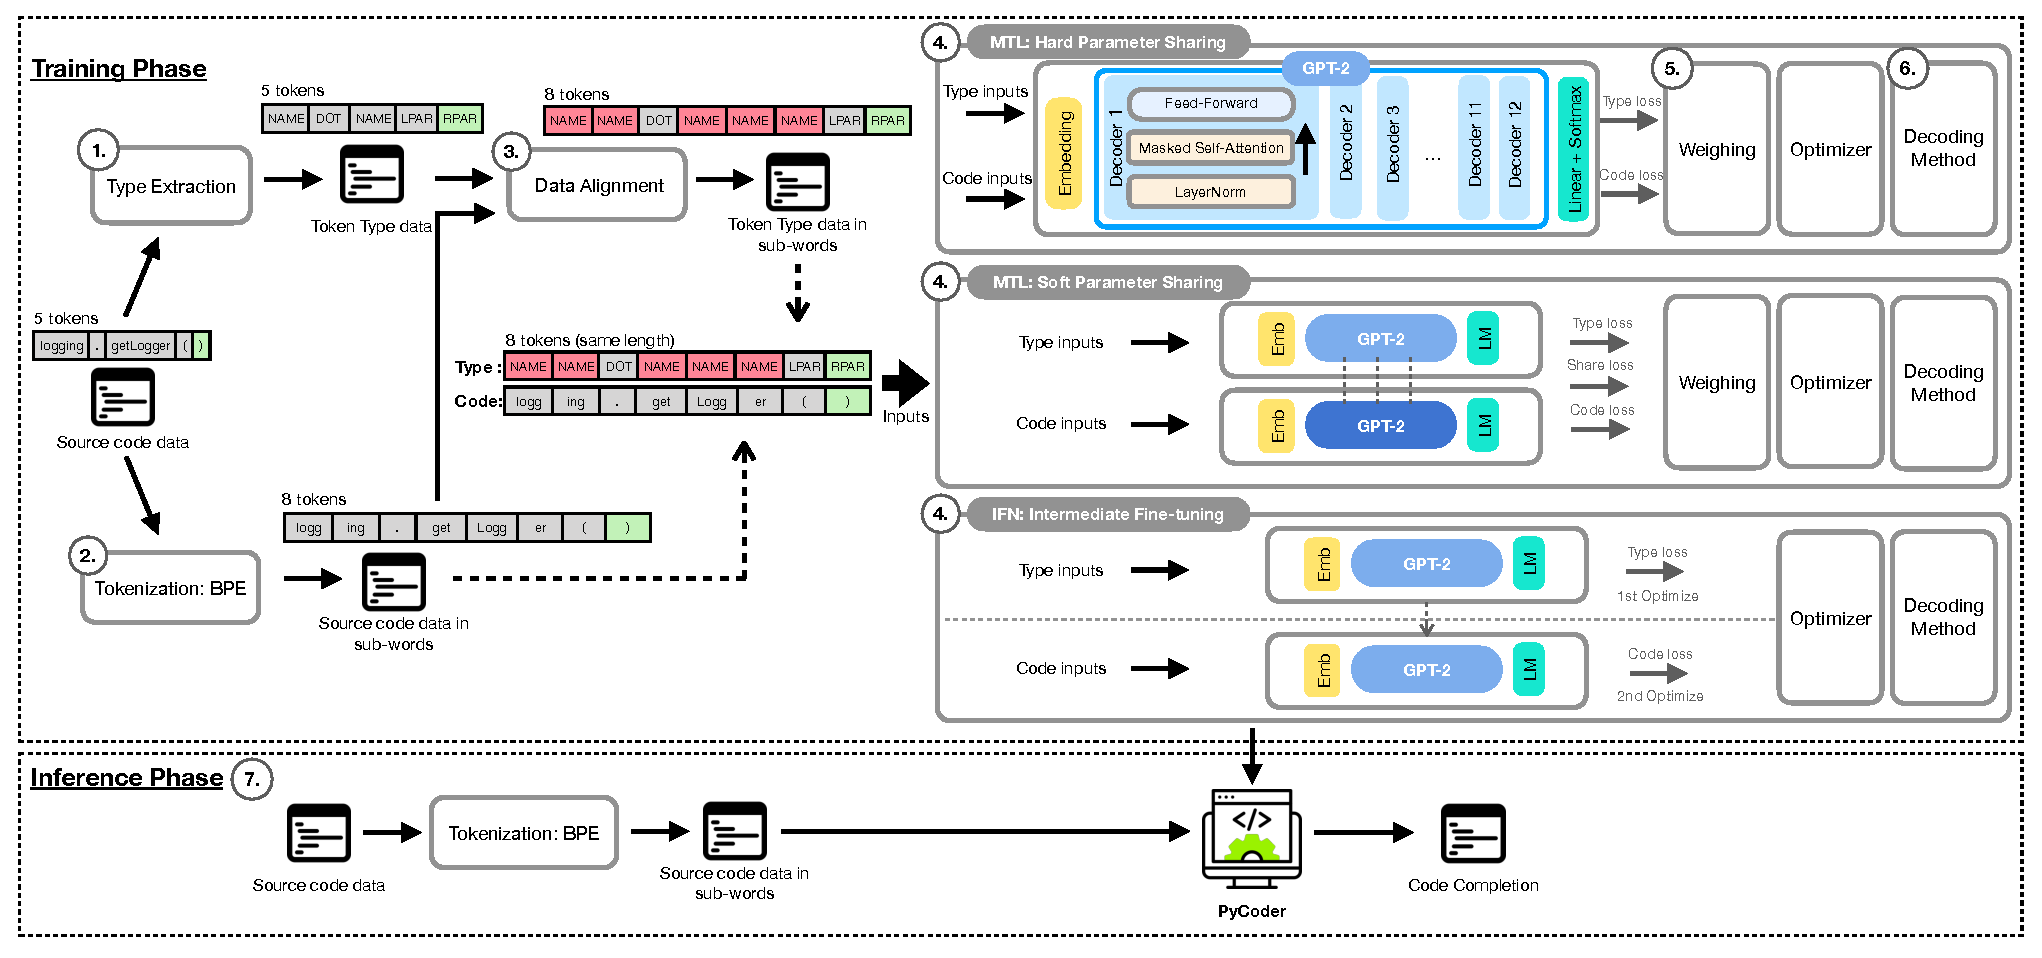
\includegraphics[width=\textwidth]{figures/overview.pdf}
    \caption{
    % \kla{An} \kla{o}verview of our \kla{syntactic-aware on-the-fly code completion} approach (\kla{SynComp})\kla{.} \kla{add a full stop in the caption everytime.} \kla{remove tag when reading this one.} \kla{This figure is nicely presented. Well done! Looks very neat.}
    An overview of our Syntax-Aware On-the-Fly Python Code Completion approach (PyCoder). 
    % \kla{can you use 1,2,3 instead of 3.1, 3.2, 3.3? Thank you.}
    }
    \label{fig:overview}
\end{figure*}

\subsection{(Step 1) Type Extraction}

Syntactic information can be represented in many forms, e.g., Abstract Syntax Tree (AST) which is widely used in the previous work, and Token Type information which remains largely unexplored.
In fact, both AST and token type information have their own advantages and disadvantages.
While AST provides a formal representation of syntactic information of source code, it requires syntactically correct source code in order to be successfully parsed by a Python AST parser.
Since our finding in Section~\ref{sec:motivation} shows that the Python AST parser failed to execute for every two out of three characters that developers type, the usage scenarios of the existing AST-based code completion approach are still limited in practice.

To address this challenge, we leverage a standard Python token type information, offering a more abstract representation of the syntactic structure of source code (e.g., Name, String, Number), which (1) is more lightweight, (2) follows the natural order of code sequences; and (3) can be successfully parsed at any times without requiring the complete and syntactically correct source code.
Generally, the standard Python token consists of two pieces of information i.e., (1) the token type, which provides syntactic meaning, and (2) the token value, which provides semantic meaning.
% Thus, each token is a substring that has semantic meaning in the grammar of the Python programming language.\footnote{https://www.asmeurer.com/brown-water-python/intro.html}
For example, given a \texttt{logging} token, the token type is \texttt{NAME} and its value is \texttt{logging}.
Since the token type information is not available in the existing code completion benchmark, we describe the steps to extract the type information below.





% The definition of a token for this tokenizer is a substring that has semantic meaning in the grammar of python language 4; thus, every token extracted by this tokenizer has a type (i.e. token type)








% To address the limitation, the token type information from a standard python tokenizer is leveraged in this work. The definition of a token for this tokenizer is a substring that has semantic meaning in the grammar of python language 4; thus, every token extracted by this tokenizer has a type (i.e. token type). Unlike AST, this token type information can be extracted at any points in source code, and can handle the invalid source code. Only the case that user has not finished typing the whole last word that the type information of the last word could return incorrectly. However, the rest of the token type information will still be able to accurately achieve






% - token type - pros - lightweight - abstracted 
% cons - not syntactically correct guaranteed like AST when generate
% - natural order of source code 


% While AST provides a formal representation of 


% AST - type and value

% correct type, wrong value -> generated code is syntactically correct, but incorrect predictions

% incorrect type, correct value -> generated code is (i.1 instead of i=1) due to incorrect type prediction.


% - AST  - cons - it requires syntactically correct source code all the time.
% - pros, generate syntactically correct nodes all the time

% given source code-> code to AST -> AST is fed into the model -> model learn to generate a new node -> producing a tree with a new node -> this tree can be parsed back to a sequence of source code, for code completion - 

% code and AST is inter-parsability

% 2/3 --- failed

% incorrect node prediction -> wrong tree -> wrong code completion

% correct node prediction, incorrect value prediction -> correct tree, but wrong code, but executable.










% Type information plays an important role in teaching model to learn the syntactic information.
% Since the benefit behind the types is to categorize the unstructured data of natural text in source code (e.g. different variable naming) into discrete groups.
% These discrete groups arranged together in sequences could represent the structures of source code, i.e. syntactic information.
% In previous works, AST type has been widely used for syntactic information; however, as discussed earlier  (section 2.2), AST is not on-the-fly information.

% To address the limitation, the token type information from a standard python tokenizer is leveraged in this work.
% The definition of \emph{a token} for this tokenizer is a substring that has semantic meaning in the grammar of python language~\footnote{https://www.asmeurer.com/brown-water-python/intro.html}; thus, every token extracted by this tokenizer has a type (i.e. token type).
% Unlike AST, this token type information can be extracted at any points in source code, and can handle the invalid source code.
% Only the case that user has not finished typing the whole last word that the type information of the last word could return incorrectly. 
% However, the rest of the token type information will still be able to accurately achieve.


To extract type information, we use the \texttt{tokenizer} function provided by the standard Python tokenizer library\footnote{https://docs.python.org/3/library/tokenize.html} with an option \texttt{exact\_type} in order to extract the most fine-grained type for each token.
For the Python tokenizer (Python 3.7 version), there will be a total of 58 different types.
In particular, we focus on the 12 primary types of code tokens as follows: \texttt{<NAME>}, \texttt{<NUMBER>}, \texttt{<STRING>}, \texttt{<INDENT>}, \texttt{<DEDENT>}, \texttt{<ERRORTOKEN>}, \texttt{<ENDCODING>}, \texttt{<ENDMARKER>}, \texttt{<COMMENT>}, \texttt{<NL>}, \texttt{<NEWLINE>}, and \texttt{<OP>}, where the \texttt{<OP>} type consists of the remaining 46 operational types (e.g., operator. delimiter), such as \texttt{<LESS>}, \texttt{<GREATER>}, \texttt{<EQUAL>}, \texttt{<DOT>}.
Then, we perform the following pre-processing steps.

\begin{itemize}
    \item First, we discard the following three token types that will not be executed, i.e., \texttt{<ENCODING>} which describes the encoding of the Python file, \texttt{<ENDMARKER>} which describes the end position of the Python file, and \texttt{<COMMENT>} which describes the code comment of the Python file.
    \item Second, \texttt{<NAME>} provided by the Python tokenizer could be either identifier names (e.g., \texttt{logging}) or Python reserved names (e.g., \texttt{True}).
    Thus, a code completion approach may not be able to recognize the difference between the identifier names and the Python reserved names---which does not reflect the reality.
    To ensure that our code completion approach can recognize the difference between different types of names, we use the \texttt{keyword.iskeyword()} function\footnote{https://docs.python.org/3/library/keyword.html} in order to check and rename all of the Python reserved words which is originally extracted as  \texttt{<NAME>} to \texttt{<KEYWORDS>}. 
    \item Third, since the CodeXGLUE~\cite{lu2021codexglue} benchmark dataset treats any new line equally, we also convert  \texttt{<NEWLINE>} (a new line), \texttt{<NL>} (a new blank/comment line) as \texttt{<EOL>} (the end of line).
\end{itemize}


With this approach, the representation of the token types (i.e., each token has its own type) follows the natural order of source code, not the AST structure which addresses the limitations of the AST-based code completion approaches.
As shown in Figure~\ref{fig:overview},  \texttt{logging.getLogger()} will be tokenized as \texttt{[logging, ., getLogger, (, )]} with the following token types \texttt{[NAME, DOT, NAME, LPAR, RPAR]}.






% extracting token-by-token in source code order, the token type information can solve limitation of AST abstract node order and perfectly fit with the natural order of the corresponding source code.




% Then, 


% Generally, reserved words or \emph{keywords} in python will be return as NAME type from tokenizer lib. We transform them to be KEYWORD type checking by keyword lib\footnote{https://docs.python.org/3/library/keyword.html}. 


% We also transform NL and NEWLINE types to EOL to be consistent with standard when ending a line.



%  We process each type by the following methods:
%     \begin{itemize}
%         % \item \textbf{Discard} : We discard the following types , ENDMARKER, COMMENT in order to focus only to the source code.
        
        
%         \item \textbf{Transform} : Generally, reserved words or \emph{keywords} in python will be return as NAME type from tokenizer lib. We transform them to be KEYWORD type checking by keyword lib\footnote{https://docs.python.org/3/library/keyword.html}. We also transform NL and NEWLINE types to EOL to be consistent with CodeXGLUE~\cite{lu2021codexglue} standard when ending a line.
        
        
        
        
%         \item \textbf{Filter} : We filter ERRORTOKEN type that has the corresponding code token as empty string.
% ""

% a=""

% a = 
% NAME, EQUAL, ERRORTOKEN



        
        % \item \textbf{Preserve} : We preserve all the rest which are INDENT, DEDENT, STRING, NUMBER and all the operational types.
        % \item \textbf{Masked sensitive data} : We apply the same methods from CodeXGLUE \cite{lu2021codexglue} to masked the sensitive data of type STRING and NUMBER in source code data.
    % \end{itemize}
    
    % After processing, the type dataset has 54 types consist of 8 primary types and 46 operational types.
    % Then the types are transformed into the placeholder $\langle$~\emph{type}~$\rangle$. For instance, NAME type will be represented as $\langle$NAME$\rangle$.
    % The example list of the final types with placeholders are shown below.
    
    % Primary types:
    % \texttt{<NAME>, <KEYWORD>, <NUMBER>, <STRING>, <INDENT>, <DEDENT>, <ERRORTOKEN>, <EOL>}
    
    % Operation types:
    % \texttt{<LPAR>, <RPAR>, <LSQB>, <RSQB>, <COLON>, <COMMA>, <SEMI>, <PLUS>, <MINUS>, <STAR>, <SLASH>, <VBAR>, <AMPER>, <LESS>, <GREATER>, <EQUAL>, <DOT>,} etc.


% name convert to keyword=  python specific keywords


% NL and NEWLINE

% There are two kinds of token types, i.e., the primary type and the operational type.
% The primary type describes the object types (e.g. Name, String, and Number) of the tokens.
% On the other hand, the operational type is for an operator, delimiter, or ellipsis literal token (e.g. plus, comma, parenthesis, and dot).




   

    
% \begin{itemize}
%     % \item \kla{I feel this could be part of the approach called data collection / to make the work more contributions. normally, anything in the experimental design will be on a standard basis. nothing new.} 
%     \item \textbf{Token Type Dataset} 
%     To extract type dataset from source code, we use the standard python tokenizer library\footnote{https://docs.python.org/3/library/tokenize.html} and the \emph{exact type} defined by the library.
%     % Unlike AST, this token type information can be extracted at any points in source code, and can handle the incomplete or invalid source code.
%     % Only the case that user has not finish typing the whole last word that the type information of the last word could return incorrectly. 
%     % However, the rest of the type information will still be able to accurately achieve.
%     % \textit{Finish} \kla{what are the benefits of this type, how does it differ from AST types? and what information that this type offer? how many types are extracted? which types do we choose? which types do we ignore? and why? what is the reason behind it?}
%     Originally there are 58 types in total (Python 3.7) which are 12 primary types, and 46 operational types.
%     We process each type by the following methods:
%     \begin{itemize}
%         \item \textbf{Discard} : We discard the following types ENDCODING, ENDMARKER, COMMENT in order to focus only to the source code.
%         \item \textbf{Transform} : Generally, reserved words or \emph{keywords} in python will be return as NAME type from tokenizer lib. We transform them to be KEYWORD type checking by keyword lib\footnote{https://docs.python.org/3/library/keyword.html}. We also transform NL and NEWLINE types to EOL to be consistent with CodeXGLUE~\cite{lu2021codexglue} standard when ending a line.
%         \item \textbf{Filter} : We filter ERRORTOKEN type that has the corresponding code token as empty string.
%         \item \textbf{Preserve} : We preserve all the rest which are INDENT, DEDENT, STRING, NUMBER and all the operational types.
%         % \item \textbf{Masked sensitive data} : We apply the same methods from CodeXGLUE \cite{lu2021codexglue} to masked the sensitive data of type STRING and NUMBER in source code data.
%     \end{itemize}
    
%     After processing, the type dataset has 54 types consist of 8 primary types and 46 operational types.
%     Then the types are transformed into the placeholder $\langle$~\emph{type}~$\rangle$. For instance, NAME type will be represented as $\langle$NAME$\rangle$.
%     The example list of the final types with placeholders are shown below.
    
%     Primary types:
%     \texttt{<NAME>, <KEYWORD>, <NUMBER>, <STRING>, <INDENT>, <DEDENT>, <ERRORTOKEN>, <EOL>}
    
%     Operation types:
%     \texttt{<LPAR>, <RPAR>, <LSQB>, <RSQB>, <COLON>, <COMMA>, <SEMI>, <PLUS>, <MINUS>, <STAR>, <SLASH>, <VBAR>, <AMPER>, <LESS>, <GREATER>, <EQUAL>, <DOT>,} etc.
%     % <PERCENT>, <LBRACE>, <RBRACE>, <EQEQUAL>, <NOTEQUAL>, <LESSEQUAL>, <GREATEREQUAL>, <TILDE>, <CIRCUMFLEX>, <LEFTSHIFT>, <RIGHTSHIFT>, <DOUBLESTAR>, <PLUSEQUAL>, <MINEQUAL>, <STAREQUAL>, <SLASHEQUAL>, <PERCENTEQUAL>, <AMPEREQUAL>, <VBAREQUAL>, <CIRCUMFLEXEQUAL>, <LEFTSHIFTEQUAL>, <RIGHTSHIFTEQUAL>, <DOUBLESTAREQUAL>, <DOUBLESLASH>, <DOUBLESLASHEQUAL>, <AT>, <ATEQUAL>, <RARROW>, <ELLIPSIS>}
    
%     % \item \textbf{Source Code Dataset} We apply the same methods from CodeXGLUE \cite{lu2021codexglue} to masked the sensitive data of type STRING and NUMBER in source code with placeholders.
%     % In addition, we preserve the indentation of the dataset which CodeXGLUE pre-processing process discards.
%     % Because it keep the details of the data.
%     % and makes the dataset be more compilable (success to parse to AST). The comparation of parsing rate \kla{unclear the parsing rate: parse for Type or for AST? I thought we will not use AST so it should not be parsed for AST.} for the test set is shown in table \ref{tab:parsing rate}
%     % We discard the indentation only when training the model for CodeXGLUE competition in RQ1.
    
% \end{itemize}

%  \kla{have we discussed about the special tokens so they will not be splitter into subword?} \textit{Gam: will mention in tokenization}

\subsection{(Step 2) Tokenization}
% Generally, source code is a sequence of code tokens where each token has its own semantic meaning.
% \gam{} Therefore, 
Tokenization is an important step in automated code completion, aiming to split the source code into meaningful units.
There are three general levels of granularity, i.e., a word level, a subword level, and a character level.
While the word-level representation is the simplest tokenization approach, it may produce a massive vocabulary size. 
However, limiting the vocabulary size based on its frequency may cause an Out-of-Vocabulary words (OOV) problem.
While the character-level representation can diminish the OOV problem with the limited vocabulary size (e.g., English characters), models may not be able to handle an excessively long sequence of source code (i.e., each character has its own vector).
Instead, we use sub-word tokenization with the Byte-Pair Encoding (BPE) algorithm~\cite{sennrich2015neural}, as prior studies found that BPE can substantially reduce the vocabulary size~\cite{fu2022gpt2sp, karampatsis2020big}, while being able to generate new identifiers that never appear in the dataset~\cite{thongtanunam2022autotransform}.
First, BPE splits source code into characters.
Then, BPE iteratively merges the characters into subwords based on the frequency of the occurrences to create the vocabulary until the desired size.
In this paper, we use the CodeGPT tokenizer, which has a vocabulary size of 50,000 subwords.
To ensure that the CodeGPT tokenizer can recognize the token types, we represent the token types in the bracket parenthesis form $\langle...\rangle$, which are included in the special token vocabulary for the BPE tokenizer to avoid any subword tokenization on these token types.
% In total, our vocabulary size is 50,288.



% Such method make BPE able to handle any new words that may appear in the future.
% The SynComp's vocabulary size for BPE method is set to 50,000.
% Additionally, we include all the placeholders for token types (section 3.1), and placeholders for masked sensitive data (section 4.2) as \emph{special tokens} in the vocabulary. 
% Thus, the placeholders are not split into sub-words when performing tokenization.
% Overall, the final size of SynComp's vocabulary is 50,288.


% be tiny and handle the OOV problem; nonetheless, there is a trade-off with the oversized input sequence length.
% The word-level tokenization is the most simple method; however, it may lead to a massive vocabulary size and one of the most important problems for tokenization step, the unknown words or Out-of-Vocabulary words (OOV) problem.
% On the contrary, the character-level tokenization can diminish the vocabulary size to be tiny and handle the OOV problem; nonetheless, there is a trade-off with the oversized input sequence length.

% to ensure that the models can learn the smallest unit of code tokens with their own meaning.


% To ensure that a code completion approach can generate the most meaningful vector representation for each token, 

% Intuitively, code tokens have their own semantic meanings. 
% Thus, 




% Tokenization step split the text data into small units and encode before inputting into the models.
% These small units can be either words, sub-words, or characters which benefit differently.
% The word-level tokenization is the most simple method; however, it may lead to a massive vocabulary size and one of the most important problems for tokenization step, the unknown words or Out-of-Vocabulary words (OOV) problem.
% On the contrary, the character-level tokenization can diminish the vocabulary size to be tiny and handle the OOV problem; nonetheless, there is a trade-off with the oversized input sequence length.
% To address these problems, SynComp performs the sub-word tokenization which exploiting word segmentation to handle unknown word and optimize the vocabulary size.
% To provide the inputs to the model, the data need to be tokenized and encoded into words or sub-words.
% One of the most important problems for this step is the unknown words or Out-of-Vocabulary words (OOV).
% To solve this problem, we choose sub-word level tokenization which is more flexible for unknown word combination in this work.
% Since our model backbone is GPT-2 with CodeGPT checkpoint (section 3.4), we adapt the tokenizer from CodeGPT~\cite{lu2021codexglue}.
% The source code inputs are encoded by Byte-Pair-Encoding (BPE) technique~\cite{sennrich2015neural}. 
% The algorithm iteratively merges the characters or character sequences by the frequency of occurrences to create the vocabulary until the desired size.
% Such method make BPE able to handle any new words that may appear in the future.
% The SynComp's vocabulary size for BPE method is set to 50,000.
% Additionally, we include all the placeholders for token types (section 3.1), and placeholders for masked sensitive data (section 4.2) as \emph{special tokens} in the vocabulary. 
% Thus, the placeholders are not split into sub-words when performing tokenization.
% Overall, the final size of SynComp's vocabulary is 50,288.

% \textit{finish} \kla{what are the existing tokenization approaches? why BPE is chosen? why others are not chosen e.g., sentencepiece? or word level? any references to support the argument? why not use code abstraction?}

\subsection{(Step 3) Data Alignment}
Data alignment is an important step to ensure that the sequence of code tokens and their corresponding token types are correctly matched and aligned.
With the use of BPE, some words may be tokenized as subwords, while their type is not tokenized into the subword level, making the sequence of code tokens and the corresponding token types not correctly matched.
For example, as shown in Figure~\ref{fig:overview}, BPE splits \texttt{logging} into \texttt{[logg, ing]} with a single corresponding \texttt{<NAME>} token type.
To address this problem, we repeat the token type for any word that is split by BPE.
Therefore, in Figure~\ref{fig:overview}, the token type \texttt{<NAME>} is repeated twice in order to match the subword-level code sequence of \texttt{[logg, ing]}.
This data alignment step will produce a sequence of code tokens and their corresponding token types with the same length, which is ready to be fed into our code completion approach to learn both syntactic and semantic meanings of source code.



% The result of the data alignment step is the type dataset that consistent and has the same data length as sub-word code dataset.
% These datasets are the inputs of our multi-task training models.




 % and splits \texttt{getLogger} into \texttt{[get, Logg, er]}, respectively

 


% nonetheless, the type still be only \emph{one} NAME for each word which will shift the index of type data to be slip up.
% To solve this problem, we repeat the type of corresponding word if the word is split by BPE.

% the function name \emph{sum\_number} is split by BPE into \emph{$[sum, \_number]$} sub-words, 
% \textit{finish} \kla{what is the purpose of data preprocessing? why do we need this step? should we call processing, preprocessing, or tokenization? how are they different?}

% \kla{from a high-level perspective, what should the dataset look like? need more technical details/description}

% \textit{finish} \kla{I would not call align dataset since this is the dataset that we are going to use.}
%  step adjusts the different tasks information (i.e. code dataset and type dataset) to be in a corresponding length with one another for multi-task training models.
% In word level, our source code dataset and token type dataset are already consistent.
% However, the tokenization step separates the source code into sub-words which could cause these dataset to be lapsed.
% To train , we need the datasets for target task (source code prediction) and auxiliary task 
% \kla{auxiliary is not defined yet - fixed, mention in data collection} 
% (type prediction) to be consistent with each others.
% However, in sub-word level from BPE tokenization, these datasets could be lapsed.
% For example, in Fig.~\ref{fig:overview}, 
% the function name \emph{sum\_number} is split by BPE into \emph{$[sum, \_number]$} sub-words, 
% an object \emph{logging} and an attribute \emph{getLogger} are split by BPE method into \emph{$[logg, ing]$} and \emph{$[get, Logg, er]$} sub-words;
% nonetheless, the type still be only \emph{one} NAME for each word which will shift the index of type data to be slip up.
% To solve this problem, we repeat the type of corresponding word if the word is split by BPE.
% Therefore, in Fig.~\ref{fig:overview} the type NAME is repeated to create the aligned datasets. 
% The result of the data alignment step is the type dataset that consistent and has the same data length as sub-word code dataset.
% These datasets are the inputs of our multi-task training models.
% The example is shown in Fig. \ref{fig:align_dataset}.


% \begin{itemize}
%     \item \textbf{Tokenization} 

    % The source code input is encoded by Byte Pair Encoding (BPE) technique~\cite{sennrich2015neural}. 
    % \kla{what are the existing tokenization approaches? why BPE is chosen? why others are not chosen e.g., sentencepiece? or word level? any references to support the argument? why not use code abstraction?}
    % The algorithm iteratively merges the characters or character sequences by the frequency of occurrences to create the vocabulary.
    % Instead of using word-level tokenization, such method make SynComp able to handle the out-of-vocabulary words.

    % \item \textbf{Align Datasets} 
    
    % \kla{should not call BPE as dataset, but a data preprocessing step.} 
    % \textbf{Repeated type dataset / BPE type dataset} To train \gls{mtl} models, we need the datasets for main task and auxiliary task to be consistent with each others. For example, the code should be numerical at the same index of type NUMBER. Currently our code dataset and type dataset are consistent in word-level, however in sub-word-level from BPE, these dataset could be lapsed. Therefore, we propose repeated type dataset to solve this problem. Using BPE tokenizer to tokenize the words, we then repeating the type of corresponding word if the word is split by BPE. The algorithm of this process is shown in Algorithm~\ref{alg:repeat type dataset}. The result is the type dataset that has the same data length as code dataset when tokenized with BPE. The example is shown in Fig. \ref{fig:ex_repeated_type}.
    
    % \begin{algorithm}
    % \caption{For creating repeated type dataset}
    % \begin{algorithmic}
    % \For {i in length(predsList)}.
    %     \State $j \gets 0$
    %     \State $currentType \gets typeList[i][j]$
    %     \State $words \gets predsList[i]$
    %     \State $subwords\gets BPE(words)$
    %     \State $subwordTypes\gets list()$
    %     \For{subword in subwords}
    %         \If{isNewWord(subword)}
    %             \State $j \gets j + 1$
    %             \State $currentType \gets typeList[i][j]$
    %         \EndIf
    %         \State $subWordTypes.append(currentType)$
    %     \EndFor
    % \EndFor
    % \end{algorithmic}
    % \label{alg:repeat type dataset}
    % \end{algorithm}
% \end{itemize}

% \begin{figure}
%     \centering
%     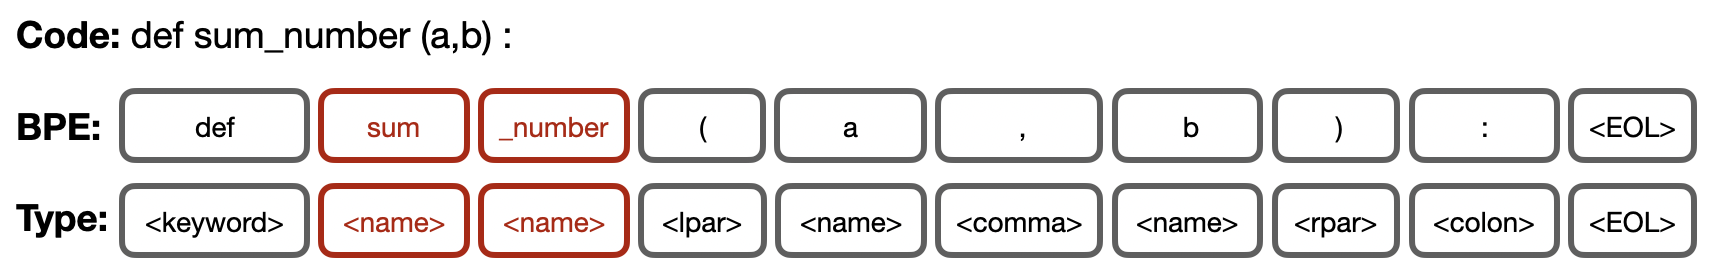
\includegraphics[width=\textwidth/2]{figures/align_dataset.png}
%     \caption{Example of align dataset}
%     \label{fig:align_dataset}
% \end{figure}

%! Author = sbbfti
%! Date = 10/06/2020

% \subsection{Models}
% \textit{finish} \kla{reviewers could argue that some other models learn both syntactic and semantic information. If this model only learns syntactic, how are they going to be accurate? check existing work why they call they learn semantic information and see if ours also learn semantic information or not. Otherwise, we are downtown the claim.}

% \kla{should we talk about two prediction tasks somewhere? Task1=? and Task2=}

\subsection{(Step 4) Multi-Task Training Architectures}
\label{sec:approach-arch}


% On the other hand, training multiple single models on multiple tasks is also possible, but predictions are competing and the multiple sources of information are not jointly learned together, leading to inaccurate predictions.



Our \our~leverages a Multi-Task Training (MTT) paradigm, which is a set of techniques designed to learn multiple tasks, allowing the model to capture multiple sources of information.
Traditionally, deep learning is designed for one single learning objective (e.g., only predicting the next code token), limiting its ability to capture other important and useful sources of information (e.g., syntactic information of source code).
Instead of training a model with one single learning objective, the MTT paradigm aims to provide a generalist model with multiple learning objectives, providing a more robust vector representation.
For our \our~approach, we design the target task to predict the next token, while the supporting task (aka. an auxiliary task or additional related non-target task) is to predict the token type.
In addition, we build three variants of \our, with three different MTT techniques, according to two learning styles~\cite{phang2018sentence} as follows.
% (i.e., \our-Hard, \our-Soft, and \our-IFN)

\subsubsection{Multi-Task Learning (MTL)}

Multi-Task Learning (MTL) is an MTT technique to learn multiple tasks simultaneously instead of learning them separately.
Normally, during the learning process, the model aims to optimize a loss function for one single learning objective.
With the MTL approaches, multiple loss functions are optimized together during the learning process, allowing the MTL-based model to simultaneously learn against multiple objectives and share the knowledge understanding from multiple related sources.
In this paper, we consider two main MTL approaches for Multi-Task Learning (MTL)~\cite{ruder2017overview}, i.e., Hard Parameter Sharing (\our-Hard) and Soft Parameter Sharing (\our-Soft).

For \emph{Hard Parameter Sharing}, the key principle is to train a code completion model against two learning objectives, where the loss functions of the two learning objectives ($L_{code}$ and $L_{type}$) are optimized together within the same model.
Formally, the \our-Hard model aims to minimize the following loss function: 
\begin{equation}
    \label{eq:1} 
    \begin{aligned}
    \medmath{L_{Hard} = \argmin_{\omega}(L_{code}(d_{code}, \omega) + L_{type}(d_{type}, \omega))}
    % loss_{hardShare} = codeLoss + typeLoss
    \end{aligned}
\end{equation} 

\noindent , where $d_{code}, d_{type}$ denotes the code token dataset and the token type dataset, respectively, and $\omega$ denotes a model's parameters.
With Hard Parameter Sharing, the weights and model parameters are shared between tasks, allowing the model to explicitly learn the input representations between tasks (i.e., code and type vectors) that are closely related.



% via the shared layers which may help enhance the effectiveness of the target task's results.
% After the shared layers, usually there are separated task-specific output layers for each task.
% However for our work, the tasks have similar outputs i.e. tokens from the vocabulary.
% Therefore, we train both target task and supporting task in the same model simultaneously without separated output layer.

% SynComp hard parameter sharing uses one GPT-2 model with two losses: code prediction loss ($L_{code}$) and type prediction loss ($L_{type}$).
% The model minimize the summation of losses shown in Equation~\ref{eq:1}.



% For hard parameter sharing, the tasks will share the same model backbone which mean the weights and parameter of the model being shared together.
% Only the task-specific output layer that might be different.
% A hard parameter sharing model is one of the most popular multi-task learning techniques.
 

% \kla{wannita will write soft....}

% \subsubsection{MTL: Soft Parameter Sharing Model}
% For soft parameter sharing, each task will have its own model backbone, i.e. separate weights and parameters.
% However, the models are loosely connected by the constraint which try to minimize the distance of the model parameters' difference.
% This is to regularize the model parameters to be similar.
For \emph{Soft Parameter Sharing}, the key principle is similar to Hard Parameter Sharing where the goal is to train a code completion model with two learning objectives.
However, instead of training a model against two tasks like the Hard Parameter Sharing model, the Soft Parameter Sharing is designed to train two individual models for each task ($L_{code}$ and $L_{type}$), allowing each model to learn separately for each task.
Therefore, each learning objective has an individual model (i.e. separated weights and parameters between the learning objectives).
% to learn and predict outputs; 
To allow the model to share the knowledge between tasks (i.e., to learn the similarities between the related parameters), a shared loss function is also used, which is computed as follows:

\begin{equation}
    \label{eq:norm}
    L_{sharing}(\omega_1, \omega_2) = 
    % ||W||_F = 
    \sqrt{\sum_{i=1}^{I}\sum_{j=1}^{J}|\omega_{1(i,j)}-\omega_{2(i,j)}|^2}
\end{equation}

% Nonetheless, the models are loosely connected by the constraint to encourage similarities between related parameters.


% The constraint ($L_{sharing}$) which is used to optimize the difference of distance between the models parameters' applies with Frobenius norm:

\noindent , where $\omega_n$ denotes the model parameters of the  learning objective $n$. Finally, the \our-Soft model aims to minimize the following loss function:

\begin{equation}
\label{eq:2}
\begin{aligned}
    L_{Soft} = \argmin_{\omega_1, \omega_2}
    &( L_{sharing}(\omega_1, \omega_2)\\ 
    &+ L_{code}(d_{code}, \omega_2)\\
    &+ L_{type}(d_{type}, \omega_1))
\end{aligned}
\end{equation}

With Soft Parameter Sharing, each learning objective has its own model parameters and weights, allowing the models to implicitly learn the input representations that might have more connection to a specific task.

% SynComp soft parameter sharing uses two GPT-2 models with three losses: code prediction loss, type prediction loss, and sharing loss. The model minimize the summation of losses shown in Equation~\ref{eq:2}.

\subsubsection{Intermediate Fine-Tuning (IFT)}

\emph{Intermediate Fine-Tuning (IFT)}~\cite{phang2018sentence} adapts a transfer learning concept (i.e., pre-training then fine-tuning) where the goal is to learn multiple tasks sequentially. First, the model is fine-tuned on the supporting task (token type prediction) followed by the target task (code token prediction), respectively.
Thus, the fine-tuned step on the supporting task can be considered the second stage of the model pre-training.
Therefore, the Intermediate Fine-Tuning (IFT) model (\our-IFT) is first trained based on an intermediate self-supervised task (token type prediction), then trained on the target task (code token prediction), allowing the model to gain knowledge on the token type prior to predicting the next code tokens.


\subsection*{GPT-2 Model Architecture}

Among the three variants of the MTT techniques (i.e., \our-Hard, \our-Soft, and \our-IFT), we use the GPT-2 architecture as a base model.
GPT-2~\cite{radford2019language} is a decoder-only Transformer model.
The GPT-2 architecture for code completion consists of three main components: the embedding layer, the decoder block, and the language model head. 
First, the embedding layer embeds the input tokens into vectors with positional encoding, allowing the model to learn the semantic meaning and the position of each code token.
Then, the embedding vectors are fed into the decoder block which contains decoder layers.
Each decoder layer includes masked self-attention layers, feed-forward neural network layers, and normalization layers.
%  It basically always scores the future tokens as 0 so the model can’t peak to future words
The masked self-attention layer indicates which tokens to focus on, while the masking approach prevents the attention mechanism~\cite{vaswani2017attention} to see the unseen tokens in the future.
% \kla{wannita will do the rest}.
% Feedforward neural nets are complex network made up an input layer that accepts information, hidden layers that capture the hidden correlations between each data point, and an output layer which transmit information.
The feed-forward neural network layer is a sophisticated network with hidden nodes to capture the related information between each data point.
% Layer normalization (LayerNorm) is a technique to normalize the distributions of intermediate layers. It enables smoother gradients, faster training, and better generalization accuracy.
The normalization layer makes the learning process more effective by enabling smoother gradients and generalized accuracy.
% The linear layer takes the output of the last decoder block and converts it to a vector whose dimensions are vocabulary size by 1. In short, it takes a lot of inputs and produces a list where each spot represents a token. The higher the number in the spot the better the chance that that token is the best pick. Softmax converts the output of the linear layer to a probability distribution
After $L$ layers of decoder, an output of the last layer is fed to the language model head, i.e. a linear layer, which converts the output to a vector whose dimensions are the same as the vocabulary size.
Lastly, the vector is converted to a probability distribution by the softmax activation function.
Formally, to predict the next token $x_t$ based on a given input sequence, GPT-2 can be represented as follows:

\begin{equation}
\begin{aligned}
    \label{eq:transformer}
    h_0 &= W_e \cdot C + W_p \\
    % \label{eq:transformer2}
    h_l &= decoder\_layer(h_{l-1}), \forall l \in [1,L] \\
    % \label{eq:transformer3}
    P(x_t) &= y_t = softmax(h_n \cdot W^T_e), t \in [0, N]
\end{aligned}
\end{equation}

\noindent, where $W_e$ is the tokens embedding matrix, $C$ denotes the context vector of tokens, $W_p$ is the position embedding matrix, $L$ is a number of decoder layers, and $N$ is the length of the sequence.
We follow the traditional language models by maximizing the log-likelihood of:

\begin{equation}
    \label{eq:log-likelihood}
    L(x_t) = \sum_i{\log P(x_i|x_1...x_{i-1}, \omega)}
\end{equation}

\noindent, where $\omega$ is the model parameters that are learned during the optimization process.
Particularly, \our~uses the pre-train CodeGPT~\cite{lu2021codexglue} that is pre-trained on the CodeSearchNet dataset~\cite{husain2019codesearchnet} as a starting checkpoint.


% Below we provide details for each training techniques.



% In Fig.~\ref{fig:overview} shows the architectures of all described models.
% During the training phase, both tasks are cooperatively trained; however, the task can separately predict in the inference phase as shown in Fig.~\ref{fig:overview}.
% In other words, the token type information is used only to support throughout the training phase requiring no token type extraction in the inference phase.
% which yield to the benefit of on-the-fly model by not requiring token type extraction in the inference phase.

% SynComp has GPT-2~\cite{radford2019language}, a Transformer decoder-only model, as a based model for all techniques.
% The based model consist of three main components: embedding layer, decoder block, and language model head. 
% Before handing that to the first block in the model, we need to incorporate positional encoding – a signal that indicates the order of the words in the sequence to the transformer blocks.



% \gls{ifn} is adapted from transfer learning paradigm which is about pre-training and then fine-tuning on target task.
% Specifically, this is the training technique for sequential training.
% The model is fine-tuned on supporting tasks and then target task respectively.
% This technique benefit the model to learn the second stage of pre-training with intermediate supervised task that might mitigate the brittleness and improve the robustness and performance of the target task~\cite{phang2018sentence}.

% In our case, SynComp intermediate fine-tuning uses one GPT-2 model with the token type prediction as the supporting task. 
% Thus, we first fine-tune our \gls{ifn} model on type dataset.
% Then we fine-tune the same model again on code prediction task.




% Recently, both MTL approaches are used in code completion.
% For example, Liu~\ea~\cite{liu2020self, liu2022unified, liu2020multi} leverage Hard Parameter Sharing, while CodeFill~\cite{izadi2022codefill} leverage Soft Parameter Sharing.




% Typically, there are two approaches for training \gls{mtl}: hard parameter sharing and soft parameter sharing~\cite{ruder2017overview}.

% Basically, the inspiration to train the tasks at the same time on one or many models with jointly conditions.
% On the other hand, \gls{ifn} is the model training technique for \emph{sequential} training.

% Specifically, the model is fine-tuned sequentially on each supporting tasks, and then the target task respectively~\cite{phang2018sentence}.

% \subsubsection{Intermediate Fine-Tuning}

% To achieve this, we consider the following three MTT training techniques~\cite{phang2018sentence}.




% Some code completion research starts to apply \gls{mtl} with different tasks and datasets~\cite{izadi2022codefill, liu2020self, liu2022unified, liu2020multi}.
% Particularly, most of the time \gls{mtl} has been used for \gls{ast} training~\cite{izadi2022codefill, liu2020self, liu2022unified} in order to learn syntactic information of source code.
% However, the source code of code completion task is usually incomplete or syntactically incorrect which leads to the limitations of extracting \gls{ast} data in practice (section 2.2).
% To address the limitations of previous works, our work
% % is the first to
% leverages \gls{mtl} with \emph{token type} information that represent the light-weight syntactic information and is more flexible to be extracted. 
% Moreover, although showing benefits in many NLP research~\cite{phang2018sentence, weller2022use, gururangan2020don}, to the best of our knowledge \gls{ifn} has never been introduced to code completion field.
% Therefore, this motivate us to include the technique to our experiment along with \gls{mtl}.







% PyCoder-Hard
% PyCoder-IFT

% However, sometimes the additional related non-target tasks (i.e. supporting task or auxiliary task) are presented with the intention of improving the target task's performance.
% When supporting task has been presented during the fine-tuning stage, there are multiple techniques to combine or alternate between these target task and supporting task -- such techniques can be called \emph{multi-task training techniques}.


% at the same time rather than separately.

% target dataset
% supporting dataset



% In the past, pre-train language model and fine-tune on target task has become the standard paradigm for NLP~\cite{raffel2020exploring} and also be adapted to many tasks in software engineering~\cite{wang2021codet5, feng2020codebert}.

% These kind of tasks are called supporting task or auxiliary task.
% However, when non-target tasks has been presented more than one


% Recently in NLP, there is a study for how to best make use of the supporting data~\cite{weller2022use}.
% Two predominant methods used are \gls{mtl} and \gls{ifn}. 
% \gls{mtl} is a model training technique for \emph{simultaneous} training.
% Typically, there are two approaches for training \gls{mtl}: hard parameter sharing and soft parameter sharing~\cite{ruder2017overview}.
% Basically, the inspiration to train the tasks at the same time on one or many models with jointly conditions.
% On the other hand, \gls{ifn} is the model training technique for \emph{sequential} training.
% Specifically, the model is fine-tuned sequentially on each supporting tasks, and then the target task respectively~\cite{phang2018sentence}.



% \subsubsection{MTL: Hard Parameter Sharing Model}
% For hard parameter sharing, the tasks will share the same model backbone which mean the weights and parameters of the model being shared together.
% Only the task-specific output layer that might be different.
% A hard parameter sharing model is one of the most popular multi-task learning techniques.
% This technique completely shares the model backbone (i.e. weights and parameters) between tasks.
% The benefit is that the model could \emph{explicitly} learn the input representations between tasks via the shared layers which may help enhance the effectiveness of the target task's results.
% After the shared layers, usually there are separated task-specific output layers for each task.
% However for our work, the tasks have similar outputs i.e. tokens from the vocabulary.
% Therefore, we train both target task and supporting task in the same model simultaneously without separated output layer. 

% SynComp hard parameter sharing uses one GPT-2 model with two losses: code prediction loss ($L_{code}$) and type prediction loss ($L_{type}$).
% The model minimize the summation of losses shown in Equation~\ref{eq:1}. where $d_{code}, d_{type}$ denotes code and type dataset respectively, and $\omega$ denotes a model's parameter.


% \begin{equation}
%     \label{eq:1} 
%     \begin{aligned}
%     \medmath{L_{hardShare} = \argmin_{\omega}(L_{code}(d_{code}, \omega) + L_{type}(d_{type}, \omega))}
%     % loss_{hardShare} = codeLoss + typeLoss
%     \end{aligned}
% \end{equation} 

% \subsubsection{MTL: Soft Parameter Sharing Model}
% For soft parameter sharing, each task will have its own model backbone, i.e. separate weights and parameters.
% However, the models are loosely connected by the constraint which try to minimize the distance of the model parameters' difference.
% This is to regularize the model parameters to be similar.
% A soft parameter sharing model has particular model backbones for each objective task, i.e. separated weights and parameters.
% Each model learns and predicts results nearly independently; to be precise, there are loosely connected by the constraint to encourage similarities between related parameters.
% More specifically, the model is trained on each task individually along with penalizing on the distance between the model parameters' difference.
% The benefit of this technique is that each task has its own model parameters, so the model \emph{implicitly} learn the input representations and might have more connection to a specific-task.
% This constraint is expressed as \emph{sharingLoss} ($L_{sharing}$). 
% In this work, we apply the square Frobenius norm in Equation~\ref{eq:norm} as the \emph{sharingLoss}.

% \begin{equation}
%     \label{eq:norm}
%     ||W||^2_F = \sum_{i=1}^{I}\sum_{j=1}^{J}|w_{i,j}|^2
% \end{equation}

% SynComp soft parameter sharing uses two GPT-2 models with three losses: code prediction loss, type prediction loss, and sharing loss. The model minimize the summation of losses shown in Equation~\ref{eq:2}.
% \begin{equation}
% \label{eq:2}
% \begin{aligned}
%     L_{softShare} = \argmin_{\omega_1, \omega_2}
%     &( L_{sharing}(\omega_1, \omega_2)\\ 
%     &+ L_{code}(d_{code}, \omega_2)\\
%     &+ L_{type}(d_{type}, \omega_1))
% \end{aligned}
% \end{equation}

% \begin{equation}
%     \label{eq:2}
%     loss = \alpha * codeLoss + \beta * typeLoss + (1 - \alpha - \beta) * sharingLoss
% \end{equation}

% \subsubsection{STILTs: Intermediate Fine-tuning}
% From pre-training on supporting task, and then fine-tuning on the target task;
% this training technique apply the same paradigm method but with many supporting tasks called auxiliary tasks.



% \kla{move from background / will revise later}
% \emph{SynComp} leverages a multi-task training model, focusing on two training tasks: source code prediction (semantics information), and token type prediction (syntactic information).
% While the code prediction is a target task, the type prediction is a supporting task.
% SynComp explores on 3 multi-task training techniques: (3.4.1)~MTL: Hard Parameter Sharing Model, (3.4.2)~MTL: Soft Parameter Sharing Model, and (3.4.3)~\gls{ifn}: Intermediate Fine-tuning Model.
% Supplementary Training on Intermediate Labeled-data Tasks Model.



% Therefore, the training phase consist of 2 tasks: source code prediction and token type prediction.
% There are multiple techniques to learn such target task (source code prediction) with auxiliary task (type prediction). However, SynComp is inspired by weller~\ea~\cite{weller2022use} to leverage the usage of \gls{mtl} and \gls{ifn} training techniques. 

% \kla{why these three types are chosen? why do we need to explore these? - could cited~\cite{weller2022use} in the previous paragraph be the reason?}

% There are two dominant approaches in \gls{mtl} which are \emph{(3.3.1) hard parameter sharing model} and \emph{(3.3.2) soft parameter sharing model}. The core idea of both techniques is to learn the hidden robust representations from related tasks.

% \textbf{\gls{gtt}}
% We have 2 objective tasks here. First, the main task is code prediction and second task is type prediction as the auxiliary task. Both tasks, the models learn to predict in single-token level. Therefore when using in token-level prediction, the model can be used directly. For line-level prediction, the models are the same as in token-level prediction, however, are set to prediction until stop criteria is reached.


% \textit{finish} \kla{it would be great if we can discuss the advantages/disadvantages of each model? why we use them? why others are not explored? how are they different? }

% \textit{finish} \kla{I think we haven't talked about CodeGPT yet. Why using CodeGPT, instead of GPT-2? What is the limitation of CodeGPT? }
% We decide to include this method because the evidence shows that \gls{ifn} and \gls{mtl} are competitive and useful in some different scenario. If auxiliary task is larger than the target task, \gls{ifn} tend to perform better than \gls{mtl} \cite{weller2022use}. However, our type dataset is smaller than code dataset due to the tokenization process which all types are added in as the special tokens (see session 4.2). But we still choose to train \gls{ifn} in order to test the argument on the code completion task. We don't use repeated type dataset (see session 4.1) because dissimilar to \gls{mtl}, \gls{ifn} doesn't train code and type prediction simultaneously so we would like to maintain the granularity of data as normal.

% \begin{figure}[]
%     \centering
%     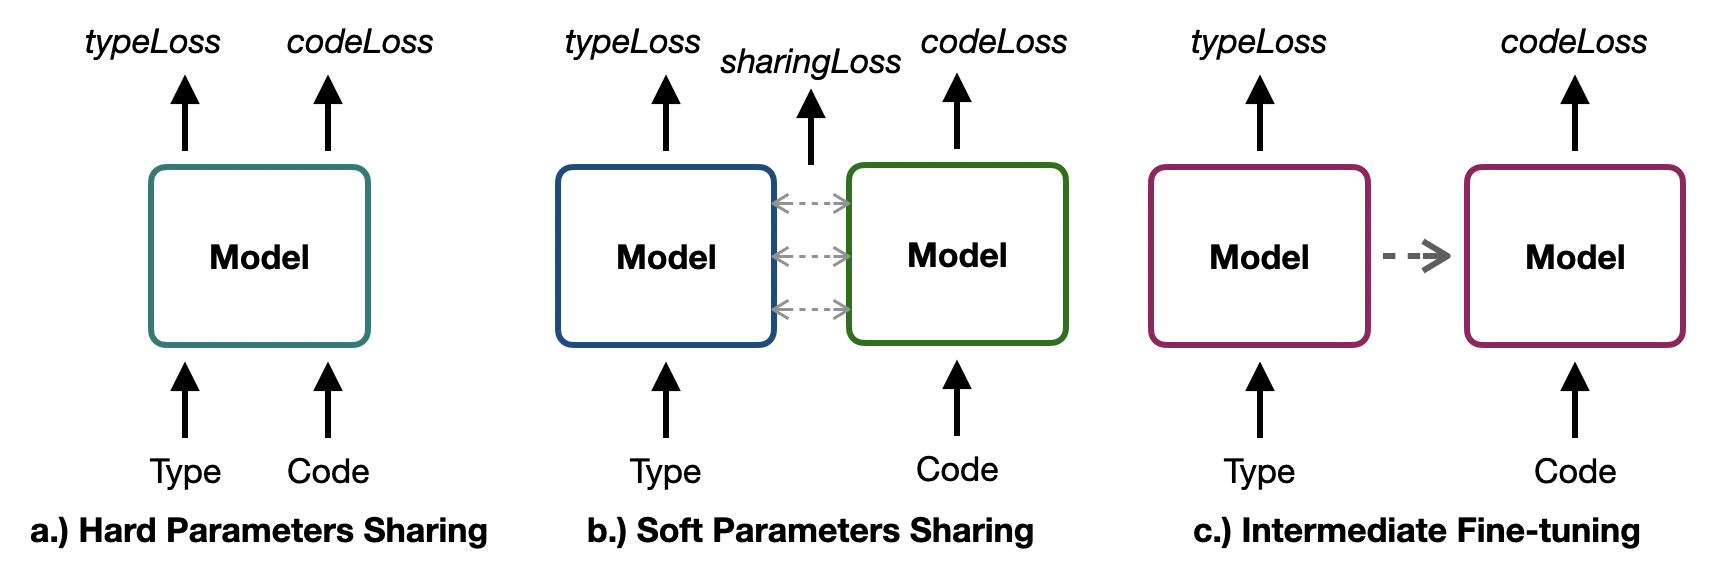
\includegraphics[width=\columnwidth]{figures/model_arch.png}
%     \caption{Model architectures (tentative pic)}
%     \label{fig:arch}
% \end{figure}

\subsection{(Step 5) Hyperparameter Task Weighting}
\label{sec:approach-weight}

Since our \our~leverages MTL training techniques to learn multiple different tasks simultaneously, some tasks may have a higher influence than others, which later may produce an unsatisfactory accuracy for the other tasks (called a conflicting gradient problem).
To prevent such conflicting gradients between tasks, it is important to find the most optimal task weights by minimizing the loss.
Therefore, we optimize the hyperparameters ($\alpha_i$) to adjust the task weights to find optimal task weights for our architecture.
Specifically, we aim to minimize the loss of the code prediction task along with the type prediction task using the following loss function.

\begin{equation}
    \label{eq:rq3}
    L_{MTL} = \argmin_{\omega}(\sum_{i}\alpha_i \cdot L_{i}(d, \omega))
    % L_{MTL} = \min_{\omega}(\alpha * L_{code}(\omega) + (1 - \alpha) * L_{type}(\omega))
    % loss = \alpha * codeLoss + (1 - \alpha) * typeLoss
\end{equation} 

% \our~performs a static weighted linear sum of losses which fixed the task's weights throughout the training phase.
% In Equation.~\ref{eq:rq3} presents SynComp's task weighing formula where $\alpha$ is the hyperparameter weight. 

\subsection{(Step 6) Decoding Methods}
\label{sec:approach-decoding}

Decoding is a method to select the next token from the potential vocabulary when generating a sequence.
Although selecting only the highest probable token is suitable for a single step, it might be a sub-optimal for the sequence.
Since the search space of the next tokens is large, different decoding methods will have different mechanisms, providing different predictions of the next tokens.
Thus, the selection of the decoding methods may have an impact on the overall performance of our ~\our.
In the code completion literature, we found that Beam Search is one of the most commonly used decoding methods.
However, Holtzman~\ea~\cite{holtzman2019curious} found that there exist other decoding methods that are widely used in the NLP area, yet remain largely explored in the code completion literature.
Thus, we aim to experiment with the six following decoding methods.

\begin{itemize}
    \item \textbf{Greedy} is a method to select the maximum probable vocabulary to be the next tokens.
    This method assumes that the model already outputs the best probability in every timestep.
    % it generates all possible tokens in the vocabulary list; then, it will choose top B candidates that have the most probability. Those B candidates will move to the next time step, and the process repeats. In the end, there will only be B candidates. The search space is only (10,000)*B.
%     Although selecting only the highest
% probability token is suitable for a specific time step, it
% might be a sub-optimal for a sequence. 
    
    \item \textbf{Beam Search} applies a search algorithm to generate all possible tokens in the vocabulary; then, it selects the top $b$ (i.e., beam size) probable tokens to continue.
    The Beam Search method is one of the most commonly used decoding methods in text generation tasks~\cite{li-etal-2016-deep, wiseman-etal-2017-challenges}.
    % However, Beam Search may not always achieve optimal results, since it does not consider the whole vocabulary, but instead only the top $b$ (i.e., beam size) probable tokens.
    % Nevertheless, Beam Search still performs faster than an exhaustive search.
    
    % ; however, it balances between the performance and the computational time.
    % The method's time complexity is equals to $O(b*V)$ where $V$ is the vocabulary size.
    % It . 
    
    % recommend the most probable $b$ next tokens according to a defined $b$ beam size threshold.

    
    
    
    % by expanding the graph in a limited set called beam~size~($b$).
    % In each timestep, the method generates all possible tokens in the vocabulary; then, it select the top $B$ probability tokens to continue.
      
    
    \item \textbf{Sampling} is a method to randomly select the next token from the actual probability distribution assigned by the model.
    Different from Greedy and Beam search methods which in some cases may recommend only the same probable next tokens at different timesteps, the sampling method may recommend different next tokens at different timesteps (i.e., non-deterministic).
    % We put the sampling method in this study as the baseline for other decoding methods. All of the methods that required sampling are set the seed value to the same number.
    
    % Temperature is used to increase the probability of probable tokens while reducing the one that is not. Usually, the range is 0 < temp ≤ 1. Note that when temp=1, there is no effect.
    \item \textbf{Sampling with Temperature} applies a temperature parameter to shape the probability distribution~\cite{ackley1985learning}, which is different from the original sampling method where the randomness is arbitrary.
    The temperature is used to increase the probability of the most probable next tokens, while decreasing the probability of the others.
    We note that the probability of the least probable next tokens is only decreased, but they are not removed from the recommendation.
    The range of the temperature value is usually at $0 < temp \le 1$, where $temp = 1$ is a normal sampling.

    % Additional to normal sampling which could be arbitrary, sampling with temperature method 
    \item \textbf{Top-K Sampling} aims to truncate the probability distribution by choosing the top-$k$ probable next tokens from the vocabulary, then, re-scale the distribution and perform sampling based on the new distribution.
    This method ensures that the less probable next tokens will not be generated, while only the top-$k$ probable next tokens are only considered during the sampling process.
    
    \item \textbf{Top-P Sampling (Nucleus Sampling)} is similar to the Top-k sampling method where the Top-P sampling method also truncates the probability distribution, but with different criteria. 
    Top-P sampling prunes the distribution by the cumulative probability of the current step $\ge p$~\cite{holtzman2019curious}; then, re-scale and perform sampling.
    Formally, given the probability P, we can define the smallest summation of the probability as $V_p$ in
    \begin{equation}
        \label{eq:top-p}
        \sum_{x\in V_p} P(x|x_{1:i-1}) \ge p
    \end{equation}
    The benefit of this method is that it can dynamically adjust the number of $k$ depending on the certainty of the model.
    If the model is very certain on some tokens, the search space is small, and vice versa.
\end{itemize}

%  the decoding method defines the way the system handles its search space over potential output utterances when generating a sequence
% The result performance in code completion may not depend only on the model, but also a method to select the output tokens from the probability distribution, i.e. a decoding method.
% The decoding method defines the way to handle the search space over potential output tokens when generating a sequence.
% Although selecting only the highest probability token is suitable for a specific time step, it might be a sub-optimal for a sequence.
% Therefore, various alternative way for decoding methods is proposed in NLP field; however, there is still a limited exploration in code completion which is similar to text generation field.
% Thus, we select 6 following decoding methods to study in this work in order to seek for the best use of our architecture.

% Even though the model leverages the token type prediction as the supporting task during the training process, at the inference phase, the model will perform only the code token prediction.
% Thus, the token type information is not required at the inference phase, allowing our \our~to perform on-the-fly code completion.



\subsection{(Step 7) Code Completion}
\our~performs predictions at two granularity levels, i.e., at the token level and at the line level.

\textbf{Token-level code completion} is a process to predict the next token (the right side), given the prior code tokens as a context (the left side).

\textbf{Line-level code completion} is similar to the token-level prediction, but the model aims to predict the next tokens until completing the whole line of code (i.e., not just only one single next token).
For the line-level prediction, we leverage the same model used for the token-level code completion task to iteratively generate the next token, where the newly generated token is used as a context for the next step of the prediction.
This process is repeated iteratively until the model generates a $\langle EOL \rangle$ token, or until it reaches a certain $n$ threshold ($n=100$, following the CodeXGlue~\cite{lu2021codexglue}).




% is occurred or the number of generated tokens become specific \emph{n} tokens, has been reach. In this work \emph{n} is set to 100.


% The task is to complete an unfinished line of code.
% Instead of training a new model, \our~adapts the token-level model for line-level prediction using a following process.
% There are 3 main steps for line-level prediction process: 1.) the model predict the next token; 2.) the predicted token is concatenated to the previous left-side context; 3.) the new sequence is recursively fed back to the model to predict the next new token.
% Firstly, the model predict the next token.
% Then, the predicted token is concatenated to the previous left-side context, and recursively fed back to the model to predict the next new token.
% This procedure performs until either one of the stop conditions, which are generating until tokens $\langle EOL \rangle$ is occurred or the number of generated tokens become specific \emph{n} tokens, has been reach. In this work \emph{n} is set to 100.
% The two stop conditions for line-level prediction are generating until tokens $\langle EOL \rangle$ is occurred, or the number of generated tokens reach n tokens.
% line-level tokens by recursively inputting the concatenation of the left-side context and the generated code.


% Specifically, as shown in the inference phase in Fig.~\ref{fig:overview}, the model receive only source code as an input in order to perform the code completion.
% Thus, \our~which has already learnt syntactic information do not need token type data for inferring, and able to remain the ability of \emph{On-the-Fly} code completion. 



   
 
    \section{Experimental Setup}\label{sec:experiment}

In this section, we present the goal of our experiment, along with the research questions, followed by the experimental setup in detail.
% We describe our python (4.1) dataset and our (4.2) pre-processing methods which are adjusted from CodeXGLUE.
% Then, we describe the details of our implementation on (4.3) model training and (4.4) evaluation measurement.
% Lastly, we explain our four state-of-the-art (4.5) baselines.
% We present: our (4.1) Dataset, which the models train and test on PY150 dataset; our (4.2) Pre-processing method, which is adjusted from CodeXGLUE.; our (4.3) Model Training, about the parameters; (4.4) Evaluation Measurement; and (4.5) Baselines, which is 4 State-of-the-art.

% We present our (4.1) Dataset, (4.2) Pre-processing Methods, (4.3) Model Training, (4.4) Evaluation Measurement, and lastly (4.5) 4 State-of-the-art Baselines.


\subsection{Goal and Research Questions}

The goal of this paper is to empirically evaluate our \our~and compare with the state-of-the-art approaches according to the token-level and line-level code completion tasks and to provide a better understanding of the impact of the components of our \our. 
To achieve this goal, we present the motivation and the research questions below.

\begin{description}
    \item \textbf{RQ1) \rqone} \\
    \textbf{Motivation.} 
    As motivated earlier, existing syntax-aware code completions are not on-the-fly, while existing on-the-fly code completions are not syntax-aware.
    To address this important gap, we introduce \our~(a syntax-aware on-the-fly code completion).
    Thus, we formulate this RQ to investigate how well our \our~perform when compared to the state-of-the-art approaches for both token-level and line-level code completion tasks based on the CodeXGlue Benchmark.
    % In this work, \our~addresses the limitations of state-of-the-art approaches as discussed in section~2.
    % In particular, 
    % instead of leverage either AST information or only source code like state-of-the-art approaches, 
    % the goal of \our~is to perform the code completion with lightweight syntax-aware information while remaining the on-the-fly feature.
    % Thus, to evaluate that our syntactic information (i.e., token type) benefit the model,
    % we formulate this RQ to compare our \our~to CodeXGLUE benchmark and four state-of-the-art approaches which include both AST and non-AST approaches.
    % and also CodeXGLUE benchmark
    \item \textbf{RQ2) \rqtwo} \\
    \textbf{Motivation.} 
    There exist various training strategies for multi-task learning used in code completion.
    For example, Liu~\ea~\cite{liu2022unified} found that hard parameter sharing performs best, while Izadi~\ea~\cite{izadi2022codefill} found that soft parameter sharing performs better than hard parameter sharing for code completion.
    % In addition, an alternate approach widely used in NLP (i.e., Intermediate Fine-Tuning) has not been explored.
    This contradictory finding motivates us to investigate the impact of training strategies on the performance of \our.
    % leaapproach; however, there are various ways available to alternate the use of supporting task (e.g., IFN and different ways to manipulate data for MTL).
    % In NLP field, Weller~\ea~\cite{weller2022use} study on these different training techniques; yet, little knowledge is known about code completion.
    % Therefore, we formulate this RQ to investigate the impact of training techniques on our \our~code completion.
    \item \textbf{RQ3) \rqthree} \\
    \textbf{Motivation.}
    Our \our~relies on two prediction tasks, i.e., code prediction and token type prediction tasks. 
    It could be possible that these two tasks may be conflicting with each other or one task has a higher influence than the other task during the learning process. 
    Thus, prior studies ~\cite{vandenhende2021multi,sener2018multi} raised concerns that the conflicting issue (aka. conflicting gradient) may degrade the performance of multi-task learning.
    Therefore, task weighting parameters are used to weigh the importance of each task to achieve optimal accuracy.
    However, \our~may be sensitive to the task weighting parameters.
    Thus, we set out this RQ to investigate the impact of the task weighting parameters on the performance of \our.
    
    
    
    
    % ensure that different tasks that are learned simultaneously have equal importance during the learning process.
    % This w
    
    
    % are an important mechanism used in multi-task learning to weigh the importance of each task during the learning process.

    
    % Prior studies~\cite{vandenhende2021multi} raised concerns that different task weighting may have an impact on the performance of the MTL models. 
    
    % This means that when training multiple tasks simultaneously, one task that is weighted more than another may have a stronger influence on the predictions than the other task, which could result in sub-optimal performance.

    
    
    % \kla{I don't get this one --- will discuss with Wannita later}
    % While MTL approach achieves success in many deep learning application, many studies mention about task weighing problem~\cite{vandenhende2021multi}.
    % In other words, when training multiple tasks simultaneously, the model may face a problem of one task dominantly influence others resulting in the sub-optimal performance.
    % To avoid this problem, the importance of task's weights adjustment has been highlighted~\cite{sener2018multi}.
    % Thus, we formulate this RQ to explore the impact of the task weighing parameters in our \our.
    \item \textbf{RQ4) \rqfour} \\
    \textbf{Motivation.}
    Decoding methods are an important component of code completion used to generate the next probably code tokens.
    Recently, only a few methods are used for code completion (e.g., Beam Search, Greedy)~\cite{svyatkovskiy2020intellicode, kim2021code, izadi2022codefill, li2017code}.
    However, there are other decoding methods that have been used for text generation in the natural language processing field, yet have never been explored in software engineering.
    Thus, there is a lack of understanding of whether decoding methods widely used in code completion are the best.
    % Many decoding methods have been proposed for , and many of them are widely adopted in software engineering.
    % Beam Search seems to be 
    % Holztman~\ea~\cite{holtzman2019curious} study on the impact of different decoding methods to generate English text; however, little knowledge has been explore on decoding methods in code completion field.
    % Specifically, most of the time only Beam search method or Greedy method is selected off-the-self~\cite{svyatkovskiy2020intellicode, kim2021code, izadi2022codefill, li2017code}.
    % Thus, we formulate this RQ to explore the impact of the different decoding methods to our \our~code completion.
\end{description}



\subsection{Dataset}\label{dataset}

We use the ETH PY150 python dataset (the standard code completion benchmark) provided by Raychev~\ea~\cite{raychev2016probabilistic} to ensure a fair comparison with prior studies ~\cite{kim2021code, izadi2022codefill, li2017code, wang2020towards}.
The dataset is collected from open-source software projects in GitHub repositories with non-viral licenses (e.g. MIT, Apache, and BSD)---a license that an owner gives permission for freely use under specific terms; thus mitigating potential licensing issues.
Note that this dataset is also used in Microsoft's CodeXGLUE benchmark~\cite{lu2021codexglue}---a worldwide competition for the AI4Code area.
As any duplicated codes have been removed by Raychev~\ea~\cite{raychev2016probabilistic}, arriving at a total of 150,000 Python files, we confirm that there is no code duplication between the training set and the testing set, thus  mitigating several potential biases like code duplication in our experiment.
% \kla{need to double check} After the authors remove duplicated files and filter only up to 30K AST nodes, the dataset contains 150,000 python source code files in total.
Following CodeXGLUE, for token-level predictions, the dataset is split into 95,000 files for the training set, 5,000 files for the validation set, and 50,000 files for the testing set, with the number of tokens of 72.1M, 4.4M, and 37.3M, respectively.
For line-level predictions, it's a common practice to reuse the same model trained for token-level predictions. 
Thus, only a testing set is required, but a training set and a validation set are not required.
Therefore, we use the 10,000 Python files provided by CodeXGLUE~\cite{lu2021codexglue} as a testing set for line-level predictions.


% For line-level dataset, there is only testing data because the model is adapted from token-level without any additional training. 

% for training and evaluation.

% It has been widely use in many code completion research~\cite{kim2021code, izadi2022codefill, li2017code, wang2020towards} and also in CodeXGLUE benchmark~\cite{lu2021codexglue}.
% We follow data split in CodeXGLUE. 
% , PY150 is 

% The numbers of tokens are 72.1M, 4.4M, and 37.3M respectively.
% For line-level dataset, there is only testing data because the model is adapted from token-level without any additional training. 

% \kla{hiding this detail may be better?}
% However, the CodeXGLUE test set does not released ground-truth data.
% But since line-level test set is a subset of token-level test set, we reconstruct the ground-truth data from CodeXGLUE samples by a following method:
% firstly, we search the inputs of line-level data in token-level data;
% then, we fulfill the ground-truths by the up coming source code, i.e. tokens on the right of inputs, until reaching $\langle EOL \rangle$ token. 

% For line-level dataset, there are no training data because the model is applied from token-level. However, the CodeXGLUE test set does also not released the ground-truth data. Thus, we reconstruct the ground-truth data from the same 10,000 testing samples in CodeXGLUE using the testing data from token-level. Since 10,000 test set in line-level is from 50,000 test set in token-level. We search the inputs of each line-level data in token-level data. Then we fulfill the ground-truth by the up coming source code until reaching $\langle EOL \rangle$ token. 
% \kla{how this part is done?} 
% Basically, randomly cutting the line and set the left side to be inputs and the rest of the line until $\langle EOL \rangle$ as ground-truths is also applicable. 
% \kla{I'm not clear this part yet.}

\subsection{Pre-processing Methods}
Sensitive data information (e.g. name, number, credential, IP address) could appear in the source code.
To avoid the models unnecessarily paying attention to this information, we mask these sensitive data by creating a placeholder for any string and numeric literals in the source code.
Particularly, following CodeXGLUE~\cite{lu2021codexglue}, we first identify tokens based on their STRING and NUMBER types.
Then, in the top-200 most frequent strings and the top-30 most frequent numeric literals, we replace the string with $\langle$STR\_LIT:\textit{value}$\rangle$ 
 and replace the number with $\langle$NUM\_LIT:\textit{value}$\rangle$.
The rest of the uncommon literals are masked by $\langle$STR\_LIT$\rangle$ or $\langle$NUM\_LIT$\rangle$.
Finally, these placeholders are also added to the special tokens of the tokenizer, avoiding any subword tokenization for these special tokens.

% the most 200 frequent

% We use CodeXGLUE~\cite{lu2021codexglue} methods to mask the literals of t with placeholders.
% Specifically, the most 200 frequent string and the most 30 frequent numerical literals are normalized in $\langle$STR\_LIT:\textit{value}$\rangle$ or $\langle$NUM\_LIT:\textit{value}$\rangle$ formats.
% The rest uncommon literals are masked by $\langle$STR\_LIT$\rangle$ or $\langle$NUM\_LIT$\rangle$.
% These placeholders are also added to the special tokens in the tokenizer; thus, they are not separated in the tokenization step (section 3.2).



% In this step, the string and numeric literals in source code dataset are normalized.
% The purposes are to mask the sensitive data that sometimes developers leave in the code  and for better training as we do not encourage the model to emphasize on different literals when predicting. 
% We use CodeXGLUE~\cite{lu2021codexglue} methods to mask the literals of token type STRING and NUMBER with placeholders.
% Specifically, the most 200 frequent string and the most 30 frequent numerical literals are normalized in $\langle$STR\_LIT:\textit{value}$\rangle$ or $\langle$NUM\_LIT:\textit{value}$\rangle$ formats.
% The rest uncommon literals are masked by $\langle$STR\_LIT$\rangle$ or $\langle$NUM\_LIT$\rangle$.
% These placeholders are also added to the special tokens in the tokenizer; thus, they are not separated in the tokenization step (section 3.2).

In addition, we preserve the original indentation of the source code that is ignored by CodeXGLUE's pre-processing step.
Indentation plays an important role as part of the Python syntax grammars, as it is used to indicate a group of statements that belongs to a particular code block, assisting a Python interpreter to decide the execution of the next statement.
To do so, for any positions of the indentation, we use $\langle$INDENT$\rangle$ and $\langle$DEDENT$\rangle$ special tokens.
$\langle$INDENT$\rangle$ denotes the indentation, which appears once at the beginning of a code block, \emph{not once per line}, while  $\langle$DEDENT$\rangle$ denotes the dedentation at the end of the code block.
% Thus, every $\langle$INDENT$\rangle$ token is matched by a corresponding $\langle$DEDENT$\rangle$ token.
% Similarly, these 
% We discard the indentation only when training the model for CodeXGLUE benchmark in RQ1 (section 5).

% assists on deciding which statement to execute next.


% Because the indentation is important in python language syntax as it assigns a group of statements to a particular block of code and assists on deciding which statement to execute next.
% We store the position of the indentation using $\langle$INDENT$\rangle$ and $\langle$DEDENT$\rangle$ tokens.
% While the $\langle$INDENT$\rangle$ token is presented once at the beginning per block of code, not once per line; the $\langle$DEDENT$\rangle$ token denotes the dedentation or the end of the block.
% Thus, every $\langle$INDENT$\rangle$ token is matched by a corresponding $\langle$DEDENT$\rangle$ token.
% We discard the indentation only when training the model for CodeXGLUE benchmark in RQ1 (section 5).

% \begin{table}[]
%     \centering
%     \begin{tabular}{l|c|c|c}
%         Dataset & Success & Indentation Error & Syntax Error \\
%         \hline
%         CodeXGLUE & 11.51 & 87.84 & 0.65 \\ 
%         Our & 88.07 & 0.00 & 11.93 \\
%     \end{tabular}
%     \caption{Compare the parsing rate between datasets.}
%     \label{tab:parsing rate}
% \end{table}

\subsection{Model Training}

% model backbone & hyperparameter -> move to model
% We use GPT-2, a decoding model consisting of 12 layers of transformers, as the based model for all our architectures.
% The warm-up checkpoint is the pre-train checkpoint from CodeGPT~\cite{lu2021codexglue} which is trained on 1.1M python function from CodeSearchNet dataset~\cite{husain2019codesearchnet}.
% Then we fine-tuned both our models and baselines on PY150 dataset. 

% tokenizer -> move to tokenization
% We adapt our tokenizer from CodeGPT. The vocabulary size for BPE method is set to 50,000.
% Additionally, the placeholders for types, and for sensitive data in strings and numbers are included in as the \emph{special tokens}. Thus, such placeholders are not split into sub-word.
% Overall, the final size of TypeComp's vocabulary is 50,288.

% For the tokenizer, we also use tokenizer from CodeGPT. The tokenizer is \gls{bpe} train for 50,000 token vocabs. The placeholder for sensitive data in strings and numbers are included in as the special tokens. Additionally, we also add all token types as the special tokens. Therefore the final size of vocabulary is 50288.

% training
We use PyTorch\footnote{https://pytorch.org}~\cite{paszke2019pytorch} and HuggingFace\footnote{https://huggingface.co}~\cite{wolf2019huggingface} libraries for the implementation of our GPT-2 based model with the pre-trained checkpoint of CodeGPT.
The base model is the default GPT-2 small configuration~\cite{radford2019language},   consisting of 12 layers of Transformer decoders, 12 attention heads, $n\_position$~=~1024, $n\_ctx$~=~1024, and $n\_embd$~=~768.
We train our models for 200,000 steps with an Adam optimizer~\cite{kingma2014adam}. 
The hyperparmeters setting is shown in Table~\ref{tab:1}.
We do not fine-tune the hyperparameters due to limited resources.
Therefore, our results could serve as a lower bound, but the optimization may improve the accuracy of our model.
Overall we train 12 variants of \our~(3 multi-task training techniques + 9 task weighing parameters) for a total of more than 850 training hours.
For the baseline, we use all the best hyperparameters described in their papers.
Our experiments is run on one NVIDIA GeForce RTX 3090 GPU with 24 GB memory, an Intel(R) Core(TM) i9-9980XE CPU @ 3.00GHz with 36 core processors, and 64G RAM.

% \kla{may be mention model training time and inference time, how many models are built, which is an approx of X GPU hours (~? days) for a commodity GPU}.

% n_positions=1024,
% n_ctx=1024,
% n_embd=768,
% n_layer=12,
% n_head=12,

% seqeunce?
% For RQ2 we compare our 3 architecture models without tasks weighing parameters.
% Then we use the best model regarding to the results from RQ2 to fine-tune tasks weighing parameters in RQ3.
% Combine results of RQ2 and RQ3, we use the best model and task weighing parameters to test for decoding methods in RQ4.
% Lastly, TypeComp, which has the best model architecture, tasks weighing parameters, and decoding method, is used to compete the state-of-the-art baselines in RQ1.

\begin{table}[]
    \centering
    \begin{tabular}{c|c}
        Hyperparameter & Value \\
        \hline
        Learning rate & 8e-5 \\
        Weight decay & 0.01 \\ 
        Batch size & 2 \\
        Gradient accumulation steps & 4 \\
        Block size for token-level & 1024 \\ 
        Block size for line-level & 924 \\
    \end{tabular}
    \caption{Model Hyperparameters.}
    \label{tab:1}
\end{table}

% During the training on \gls{mtl} models, we also have try different tasks weighing technique. The results are shown in session 5.3. 

% We improve the post-processing process from CodeXGLUE source code \footnote{https://github.com/microsoft/CodeXGLUE/tree/main/Code-Code/CodeCompletion-line}. As we observe that after finish line-predicting the existing CodeXGLUE method use function '.strip($\langle EOL \rangle$)' to truncate the $\langle EOL \rangle$ token. We found that this function doesn't remove only the given word, however every given characters from the beginning and the end of the original string \footnote{https://www.simplilearn.com/tutorials/python-tutorial/strip-in-python}. Therefore, it creates the false truncated results such as in Fig. \ref{}. 

% We propose to use '.replace($\langle EOL \rangle$,'')' for post-processing instead. Since in line-level prediction the $\langle EOL \rangle$ token is represented as the end, there will certainly have no $\langle EOL \rangle$ token in-between the results. Thus the replace function is more suitable for the truncation in this scenario. 

\subsection{Evaluation Measurement}
We evaluate our models based on the following evaluation measures: Accuracy (Acc) for token-level predictions; Exact Match (EM), Edit Similarity (ES), and Mean Reciprocal Rank (MRR) for line-level predictions.


% \our~performs two level of predictions: token-level prediction and line-level prediction. We evaluate token-level prediction with one metric: accuracy (Acc); and line-level with three metrics: exact match (EM), edit similarity (ES) and mean reciprocal rank (MRR).


% \subsubsection{Token-level prediction} %\textbf{Token-level}

\textbf{Accuracy (Acc)} is the proportion of correctness between predicted code tokens to the ground-truth tokens. 
% We use the proportion of correctness between predicted code tokens to the ground-truths as the evaluation for single token prediction. 

% \subsubsection{Line-level prediction}

\textbf{Exact Match (EM)} is similar to  Accuracy, but is evaluated at the line level, meaning that the whole predicted lines must be exactly matched with the ground-truth lines. 

% We call this measurement as exact match to be consistent with CodeXGLUE \cite{lu2021codexglue}.
% Similar to token-level prediction, we also measure the correctness (i.e., accuracy) of line-level prediction by comparing the whole predicted code line. We call this measurement as exact match to be consistent with CodeXGLUE \cite{lu2021codexglue} evaluation.

\textbf{Edit Similarity (ES)} uses a  Levenshtein distance~\cite{1966SPhD...10..707L} to measure the edit distance between the predicted lines and ground-truth lines. 
The Levenshtein distance is the minimum number of edits in characters (either an insertion, a deletion, or a replacement of a character) between the predicted line and the ground-truth line. 
% We use Levenshtein distance~\cite{1966SPhD...10..707L} to measure the edit similarity between predictions and ground-truths. The Levenshtein distance is the minimum number of edit in characters from one text to the other. The edit is defined by either an insertion, a deletion, or a replacement of a character. 

\textbf{Mean Reciprocal Rank (MRR)} evaluates the top-$R$ possible results using the multiplicative inverse of the rank of the first correct prediction. 
Formally, MRR is defined as:
% We evaluate the list of top-R possible results using multiplicative inverse of the rank of the first correct prediction. The rank is defined as:
\begin{equation}
    \label{eq:mrr}
    MRR=\frac{1}{|Q|}\sum_{i=1}^{|Q|}\frac{1}{rank_i}
\end{equation}
% \[ MRR=\frac{1}{|Q|}\sum_{i=1}^{|Q|}\frac{1}{rank_i} \]
\noindent, where $Q$ is the number of samples, and $rank_i$ is the rank of the correct prediction given by the model.
If the correct prediction exceeds rank $R$, then the reciprocal rank is 0.
In this paper, we use $R=5$.

\subsection{Baselines}

There exist various non-AST-based code completion approaches in CodeXGLUE~\cite{lu2021codexglue,radford2019language} and AST-based code completion approaches~\cite{kim2021code,izadi2022codefill,li2017code} in the literature.
To ensure that our evaluation is reasonably comprehensive, we consider a total of seven (7) baselines with respect to two evaluation settings: (1) externally evaluate the prediction results through the CodeXGLUE leaderboard,\footnote{https://microsoft.github.io/CodeXGLUE/} and (2) internally evaluate the prediction results within our own setting.

For the CodeXGLUE evaluation setting, we compare our approach with CodeGPT-adapt, CodeGPT, GPT-2, Transformer (12L), and LSTM+BPE.
To do so, we apply our \our~to the testing set provided by CodeXGLUE for both token-level and line-level predictions.
Then, the prediction results are submitted to the CodeXGLUE team to obtain the results based on their evaluation setting.

For our own evaluation setting, we consider two AST-based approaches (i.e., Pointer Mixture Network~\cite{li2017code} and TravTrans~\cite{kim2021code}); and two non AST-based approaches (i.e., GPT-2 and CodeGPT).
We do not consider CodeFill~\cite{izadi2022codefill}, since the available replication package is not executable. 
We also do not consider Codex (i.e., a descendant of GPT-3 for source code) in our experiment due to the different levels of model parameter size. 
GPT-3, a base model of Codex, has 175B model parameters, which is 100x larger than the size of our GPT-2 based model which has only 117M model parameters.
Below, we describe the details of each approach. 


% We also consider CodeFill model\footnote{https://github.com/saltudelft/codefill}
% as a baseline; however, the replication package of CodeFill is not available at the time of the experiments\footnote{We try sending an email to ask the authors, but there is still no updates on the replication package.}.





% \kla{we can even say that we compare with both AST-based and non AST-based approaches.}
% Apart from sending our model results to evaluate in CodeXGLUE benchmark~\cite{lu2021codexglue}, we compare our model with four state-of-the-art approaches to provide the concise evaluation.
% The baselines include both AST-based models: Pointer Mixture Network and TravTrans; and non AST-based models: GPT-2 and CodeGPT. 





% We run all baselines using their replication packages provided by authors. 


% The string and numerical literals in PY150 AST dataset of Pointer Mixture Network and TravTrans are masked with the similar pre-processing method to ours before the training process. 
% We also consider CodeFill model\footnote{https://github.com/saltudelft/codefill}
% as a baseline; however, the replication package of CodeFill is not available at the time of the experiments\footnote{We try sending an email to ask the authors, but there is still no updates on the replication package.}.
% \kla{codefill [AST], but the replication not available}


\begin{table*}[t]
\centering
% \resizebox{\columnwidth}{!}{
\begin{tabular}{c|l|l|l|c|c|c}
    & & & & \multicolumn{2}{c}{Line-level} & \multicolumn{1}{|c}{Token-level} \\
    \hline
    Rank & Model & Team name & Date & EM & ES & Acc \\
    \hline
    1 & \our-Hard & Monash University & 2022-10-13 & \textbf{43.91} & \textbf{71.74} & \textbf{76.93}\\
    \hline
    2 & CodeGPT-adapt & CodeXGLUE Team & 2020-08-30 & 42.37 & 71.59 & 76.60 \\
    3 & CodeGPT & CodeXGLUE Team & 2020-08-30 & 42.18 & 71.23 & 76.58 \\
    4 & GPT-2 & CodeXGLUE Team & 2020-08-30 & 41.73 & 70.60 & 75.90 \\
    5 & Transformer (12L) & CodeXGLUE Team & 2020-08-30 & 38.51 & 69.01 & 74.48 \\
    6 & LSTM + BPE & CodeXGLUE Team & 2020-08-30 & 23.77 & 56.26 & 61.94 \\
    % \hline
    % \our-Hard& \textbf{76.93} & \textbf{43.91} & \textbf{71.74} \\
\end{tabular}
% }
\caption{(RQ1) The results that appear in the CodeXGLUE leaderboard 
% as of 15 October 2022 filtered only Python
(\url{https://microsoft.github.io/CodeXGLUE/}).
% The evaluation results are calculated based on their ground-truth dataset.
% \kla{add ranking column? team name?}
% Compare results to the baseline in CodeXGLUE Benchmark. \kla{will check again after the table is revised. PyCoder to the top, sort from max to min. Double-check capitalization carefully, Make it neat, fits the table nicely to the column. add batch size column too. }
}
\label{tab:rq1 codexglue}
\end{table*}


% The evaluation results based on the CodeXGLUE leaderboard show that \our~outperform other baselines by \kla{X\%-Y\%}.

\begin{table}[t]
\centering
% \resizebox{\columnwidth}{!}{
\begin{tabular}{l|c|c|c|c}
    & \multicolumn{3}{c}{Line-level} & \multicolumn{1}{|c}{Token-level} \\
    \hline
    Model & EM & ES & MRR & Acc \\
    \hline
    \our-Hard & \textbf{43.37} & \textbf{73.20} & \textbf{48.82} & \textbf{77.12} \\
    \hline
    CodeGPT & 40.03 & 70.61 & 46.64 & 75.69 \\
    TravTrans & - & - & - & 75.50\\
    GPT-2 & 37.64 & 68.44 & 43.85 & 73.89 \\
    PMN & - & - & - & 69.02\\
\end{tabular}
% }
\caption{(RQ1) The results of \our~when compared to existing approaches through our internal evaluation.
}
\label{tab:rq1 our}
\end{table} 

\begin{itemize}
    \item \textbf{Pointer Mixture Network (PMN)}, proposed by Li~\ea~\cite{li2017code}, is an LSTM-based code completion
    % \kla{code completion--to make it context-specific, not generic LSTM model } model 
    % ?????\kla{fix the rest, same pattern as below} 
    leveraging AST information for syntactic structures.
    The model is designed with pointer networks to mitigate the OOV problems in code completion.
    % The model learns to generate the next token from either within vocabulary word or regenerate an Out-of-Vocabulary word from local context through the pointer component.
    Their replication package is available on Github\footnote{https://github.com/jack57lee/neuralCodeCompletion} and also in Pytorch version.\footnote{https://github.com/oleges1/code-completion}

    \item \textbf{TravTrans}, proposed by Kim~\ea~\cite{kim2021code}, is a transformer-based model that considers the syntactical structure of source code via AST information.
    Their replication package is available on GitHub\footnote{https://github.com/facebookresearch/code-prediction-transformer}.
    
    \item \textbf{GPT-2}, proposed by Radford~\ea~\cite{radford2019language}, is a GPT-2-based model for text generation tasks. 
    The GPT-2 model is first pre-trained on millions of English web pages (the WebText corpus) to build a language model through self-supervision learning without any explicit labels. 
    The model is available on HuggingFace.\footnote{https://huggingface.co/gpt2}
    
    % The tokenizer use in this work is BPE~\cite{sennrich2015neural}.
    \item \textbf{CodeGPT}, proposed by Lu~\ea~\cite{lu2021codexglue}, is a GPT-2-based model for source code generation.
    The CodeGPT model is a GPT-2 model that is pre-trained on a monolingual python source code from CodeSearchNet~\cite{husain2019codesearchnet} dataset.
    % \kla{CSN has many PLs. are you sure only python?}.
    The model is available on HuggingFace.\footnote{https://huggingface.co/microsoft/CodeGPT-small-py}
    
    % In CodeXGLUE benchmark dataset from Lu~\ea~\cite{lu2021codexglue} proposed baseline: CodeGPT for code generation tasks.
    % CodeGPT has the similar transformer-based model as GPT-2; however, the model is pre-trained on monolingual python source code dataset i.e. CodeSearchNet~\cite{husain2019codesearchnet}.
    % The BPE tokenizer was also newly train on source code data.
    % The model is available on HuggingFace\footnote{https://huggingface.co/microsoft/CodeGPT-small-py}
\end{itemize}

   

   \section{Experimental Results}\label{sec:results}

In this section, we present the experimental results according to our four research questions (RQs).

\subsection*{\textbf{(RQ1) \rqone}}

% \kla{Wannita, please compute the \% in the blank throughout the paper. Thanks.}


% Compare results to the state-of-the-art baselines. \kla{will check again after the table is revised. PyCoder to the top, sort from max to min. Double-check capitalization carefully, Make it neat, fits the table nicely to the column. add batch size column too. }


\indent \textbf{\our.} Among our comprehensive investigation, the best setting for \our~is to train with the hard parameter sharing strategy (\our-Hard), a task weight of 9:1 (code:type) using a Beam Search as a decoding method.
We use this setting as a reference for comparison with other approaches throughout the paper.

% \noindent \textbf{Results.} 
\textbf{\our~achieves the first rank on the CodeXGLUE leaderboard for the code completion task} (as of 13 October 2022, see Table~\ref{tab:rq1 codexglue}).
% \kla{ in the website, it shows line first, then token. for our case, there is a bigger improvement for line, than token. why don't we sell line first, then token? thought?}
We find that \our~achieves an accuracy of 76.93\% for the token-level predictions, while achieving an exact match of 43.91\% for the line-level predictions.
The evaluation results confirm that  \our~is more accurate than other baselines by 0.43\%-24.25\% for token-level predictions and 3.63\%-84.73\% for line-level predictions.
% \kla{may talk about why small improvement - could be due to batch size, limited GPU capacity, etc... at least, still outperform and}

Similarly, \textbf{\our~outperforms existing AST-based and non-AST-based code completion approaches}, according to our own setting.
Table~\ref{tab:rq1 our} shows that \our~achieves an accuracy of 77.12\% for the token-level predictions, while achieving an exact match of 43.37\% for the line-level predictions.
For the token-level predictions (Acc), we find that \our~is more accurate than Pointer Mixture Network by 11.74\%, GPT-2 by 4.37\%, TravTrans by 2.15\%, and CodeGPT by 1.89\%. 
This finding indicates that \our~that is syntax-aware and on-the-fly performs better than a code completion approach that is either syntax-aware alone or on-the-fly alone.
It is worth noting that the accuracy of \our-Hard, CodeGPT, and GPT-2 achieved for the CodeXGLUE leaderboard is slightly different from the accuracy of those that are run in our experimental setup.
The difference that we observed has to do with the dataset used in CodeXGLUE and our experiment.
In CodeXGLUE, they removed the indentation, while the dataset used in our experiment preserved the original indentation.
To mimic the practical deployment scenario, we opt to preserve the original indentation.

% \kla{will talk about the small diff value btw codexglue and our own here why}

In addition, \textbf{the token-type information can improve the line-level code completion task by 8.34\%-15.22\%.}
For the line-level predictions (EM), we find that \our~is more accurate than GPT-2 by 15.22\% and CodeGPT by 8.34\%. 
This finding indicates that the use of token-type information that is largely ignored by the literature can also improve the line-level predictions by 8.34\% to 15.22\%, confirming that the token-type information is useful to improve the performance of line-level code completions.

Finally, when comparing \our~with the existing AST-based code completions (i.e., TravTrans and Pointer Mixture Network), we find that the existing AST-based code completions are designed for the token-level predictions only.
Thus, the line-level predictions cannot be performed, highlighting the limitations of the AST-based approaches that require AST information at the inference time, while demonstrating the benefits of our approach that consider the token-type information (i.e., \emph{syntax-aware}), while can still predict code at any points of time (i.e., \emph{on-the-fly}).


% We evaluate the performance of our SynComp to complete the source code in token-level prediction and line-level prediction, compare against 4 state-of-the-art baselines and CodeXGLUE benchmark.
% \kla{do XXX.}
% We have two main results in this research question. 
% First is the results of \our~comparing with four state-of-the-art approaches implementing from their replication packages.
% Second is the results we receive from CodeXGLUE benchmark~\cite{lu2021codexglue} on code completion task.


% \our~model used in this RQ is PyCoder-Hard i.e., the MTL: hard parameter sharing with task's weight 9:1 (code:type) model which give the best experimental results from RQ~2~to~4.
% Below we provide the details of our results.

% \kla{will go from here once the table is revised.}

% \textbf{\our~on CodeXGLUE Benchmark} 
%     In Table.~\ref{tab:rq1 codexglue} shows the results of \our~in code completion task on CodeXGLUE benchmark\footnote{https://microsoft.github.io/CodeXGLUE/}.
%     Note that we run our \our~on CodeXGLUE dataset and send the predictions to CodeXGLUE benchmark for evaluation.
%     The results validate that our \our~surpasses the state-of-the-art CodeGPT and CodeGPT-adapt model, resulting in the first place in CodeXGLUE's python code completion tasks.
%     Specifically, in token-level prediction, the accuracy is relatively improved by 0.43\% %0.33\% 
%     (from 76.60 to 76.93).
%     While in line-level predictions, the exact match is relatively improved by 3.73\% %1.58\% 
%     (from 42.37 to 43.91) and the edit similarity is relatively improved by 0.21\% %0.15\% 
%     (from 71.59\% to 71.74\%).

    
% \textbf{\our~with State-of-the-art approaches} 
%     In Table.~\ref{tab:rq1} shows the results of \our~with four state-of-the-art approaches: Pointer Mixture Network~\cite{li2017code}, TravTrans~\cite{kim2021code}, GPT-2~\cite{radford2019language}, and CodeGPT~\cite{lu2021codexglue}.
%     % All state-of-the-art approaches are run from their replication packages and fine-tuning with the best hyperparameters reported in their papers.
%     The results show that our model surpass all state-of-the-art approaches.
%     Compared with second-best models, \our~achieves an improvement on accuracy of 1.89\% (from 75.69\% to 77.12\%) in token-level prediction, and on exact match of 8.34\% (from 40.03\% to 43.37\%) and edit similarity of 3.67\% (from 70.61\% to 73.20\%) in line-level prediction.
    % In token-level prediction, the accuracy is relatively improved by 1.89\% %1.43\% 
    % (from 75.69\% to 77.12\%). 
    % In line-level completion, the Exact Match is relatively improved by 8.34\% %3.34\% 
    % (from 40.03\% to 43.37\%) and edit similarity is relatively improved by 3.67\% % 2.59\% 
    % (from 70.61\% to 73.20\%). 

    

% \begin{itemize}
%     \item 

    
%     \item 
% \end{itemize}

% As a result, this can indicate that the token type syntactic information can be beneficial as a supporting data and does help enhance the performances in both token-level and line-level code completion.

% diff due to
% dataset — table3 (our) keep indentation info. , table4(codexglue) discard indentation info.
% batch size — table 4 no batch size information, but what is our?


\begin{tcolorbox}

% To answer this RQ, we build SynComp from the best combination of experiments on model technique (RQ2), task weighing parameters (RQ3) and decoding methods (RQ4) i.e. hard parameters sharing model with weighing code to type tasks as 9:1, and beam search as decoding methods.See the details of each experiment result in the following RQs.
\emph{\textbf{RQ1 Summary.} 
\fdone
% \our~surpasses all the state-of-the-art code completion models.
% The line-level exact match is improved by 8.34\%-15.22\%, while the token-level accuracy is improved by 1.89\%-11.74\%.
% \our~also receives the first place in CodeXGLUE’s python code completion benchmark. The results indicate that the token type syntactic information can be beneficial as a supporting data.
}
\end{tcolorbox}

% \subsection{RQ2: What is the impact of the training strategies on the performance of our approach}
\begin{table}[t]
    \centering
    % \resizebox{\columnwidth}{!}{
    \begin{tabular}{l|c|c|c|c}
        & \multicolumn{3}{c}{Line-level} & \multicolumn{1}{|c}{Token-level}\\
        \hline
        Model & EM & ES & MRR & Acc \\%& Type Acc \\
        \hline
        \our-Hard & \textbf{42.83} & \textbf{72.82} & 48.42 & \textbf{77.00} \\ %& \textbf{82.49} \\
        \our-IFN & 42.04 & 71.92 & \textbf{48.54} & 76.52 \\ %& 0.0 \\
        \our-Soft & 38.29 & 69.11 & 44.66 & 74.77 \\ %& 80.68 \\
    \end{tabular}
    % }
    \caption{(RQ2) The results of \our~when using various multi-task training strategies. For a fair comparison with other multi-task training strategies, we do not put any weights between tasks on \our-Hard (i.e., \emph{No Weight}).
    % \kla{I feel type acc should be dropped. irrelevant, and never talked about it before.}
    }
    \label{tab:rq2}
\end{table}

% To answer this research question, we compare the best results of each model techniques after tuning weighing (see session 5.3). The results are shown in Table \ref{tab:rq2}. From the table, hard parameters sharing with manual weight of 9:1 perform the best in both token-level and line-level prediction. This is also the method we decide to use sending results to CodeXGLUE competition. Second place is \gls{ifn} method. Even though \gls{ifn} method give comparable results to hard parameters sharing model. When we train further to the optima, the \gls{ifn} model are struggled on forgetting catastrophe \cite{} which cause the model to perform worse than hard parameters sharing later.   

% if no-weight results -> write about even if IFN is slightly better but when training further the results drop because of the forget catastrophe

% \textbf{Approach.} To answer this research question, we compare the results of each model training techniques: hard parameters sharing (MTL), soft parameters sharing (MTL), and intermediate fine-tuning (STILTs); before tuning the task weighing parameters. 

\subsection*{\textbf{(RQ2) \rqtwo}}

Table~\ref{tab:rq2} presents the results of \our~when using various multi-task training strategies.

\textbf{Hard parameter sharing (\our-Hard) as a multi-task training strategy performs the best.}
Table~\ref{tab:rq2} shows that different multi-task training strategies have an impact on the performance of \our~for both token-level and line-level predictions.
Particularly, we observe that \our~with hard parameter sharing achieves an exact match of 42.83\%, while \our~with software parameter sharing achieves an exact match of 38.29\%. 
The 4.54\% difference (i.e., max-min) confirms the impact that the training strategies have on the performance of \our.
In addition, our results are contradictory to Izadi~\ea~\cite{izadi2022codefill} who found that soft parameter sharing performs best for code completion.
% , while being in line with Liu~\ea~\cite{liu2022unified} who found that hard parameters sharing performs best.
This finding highlights the importance of investigating various choices of multi-task training strategies for code completions, instead of following prior suggestions or practices.

Different from Izadi~\ea~\cite{izadi2022codefill}, our \our-Hard is designed to take both sequences of code tokens and their types as inputs one-by-one at a time and simultaneously learn with the same loss functions that are optimized together within the same model.
With this method, the inputs can be detached from each other at the inference phase, resulting in better performance confirmed by our results.
Nonetheless, the high-performing hard parameter-sharing training strategy (\our-Hard) has to do with the benefits of the tight relationship between the learning tasks (i.e., code predictions and type predictions).
Since token types are directly aligned with the same sequence of code tokens, these two pieces of information have a tight relationship.
Therefore, \our-Hard, which completely shares the model’s weights and parameters between tasks, gains the most benefit from the shared relationship between the code and type information.
However, the soft parameter sharing model (\our-Soft) learns each task separately, making the learning process between two related tasks harder, resulting in sub-optimal performance.

% Our \our-Hard~is designed to take both sequences of code tokens and their types as input and simultaneously learn with the same loss functions that are optimized together within the same model.
% With this method, the model will be able to learn the syntactic information from types in the training phase without requiring types in the inference phase as the inputs can be detached from each others.
% The results in Tables~\ref{tab:rq2} show that this hard parameter sharing model -- \our-Hard performs the best in our case.
% \kla{why this is great?}

% Our \our-IFN~is designed to learn all sequence of types and then code tokens separately. 
% Thus, similar to \our-Hard, \our-IFN  is also able to predict without types in the inference phase as the tasks are learnt separately but sequentially within the same model.
% The results in Table~\ref{tab:rq2} show that this intermediate fine-tuning model -- \our-IFN performs as the second place in our case.
% However, we observed the type accuracy in token-level prediction and found that type accuracy of \our-IFN go down to 0\%.
% As a results, it shows that the model faces prevalent problems when training a model sequentially: a catastrophic forgetting~\cite{mccloskey1989catastrophic, kaushik2021understanding}.
% In other words, \our-IFN has already forgotten the token type information which is the reason of the worse results than \our-Hard which can access the type data all along the training.

% Our \our-Soft~is designed to take sequences of code tokens and types to learn in separated models, then optimizes simultaneously with the loosely joint to share knowledge between the models.
% Therefore, although being trained together, the model can be used separately in the inference phase allowing the prediction without type inputs.
% The results in Table~\ref{tab:rq2} show that the soft parameter sharing model -- \our-Soft performs as the last in our case.

% \kla{need to discuss/explain why hard is better than soft, why soft is worst?}

% \textbf{Results.} 
% The results are presented in Table~\ref{tab:rq2}.
% indicating that the different multi-task training techniques can vary the results as follows.
% In token-level prediction, the accuracy can be relatively different by 2.98\% %2.23\%
% (from 74.77\% to 77.00\%), and in line-level prediction, the exact match is relatively different by 11.86\% %4.54\% 
% (from 38.29\% to 42.83\%), the edit similarity by 5.37\% %3.71\%
% (from 69.11\% to 72.82\%) and the mean reciprocal rank by 8.69\% %3.88\% 
% (from 44.66\% to 48.54\%).
% In particular, we can observe that the best multi-task training technique in our setting is the \emph{MTL: hard parameters sharing model} (\our-Hard), which give the highest score in both token-level prediction (accuracy=77.00\%) and line-level prediction (exact match=42.83\%).
% This is contrast to a recent study of Izadi~\ea\cite{izadi2022codefill} which propose CodeFill with soft parameters sharing model over hard parameters sharing model.

% However, it is worth noting that different from CodeFill which the input is the concatenation of type and token, our hard parameters sharing model feeds inputs separately while optimizing together.
% On the contrary, the worst model are the \emph{MTL: soft parameters sharing model} (\our-Soft), which in this comparison give the lowest scores in both token-level prediction (accuracy=74.77\%) and line-level prediction (exact match=38.29\%).
% The explanation for these gaps might be because the token type information is a lot correspondent to the source code from which the types directly extracted and aligned in sequences.
% Thus, the hard parameters sharing model, which completely shares the model's weights and parameters between tasks, is reasonable improving the performance; however, the soft parameters sharing model which learn each task separately might be more struggle to relate the tasks.

% Additionally, we also show the accuracy of token-level prediction for token types in Table.~\ref{tab:rq2} which clearly emphasizes the different between MTL and IFN. 
% Even though the results of IFN model for code completion is comparable to the one produced by hard parameters sharing model with difference by 0.63\% (from 76.52\% to 77.00\%) in the token-level prediction accuracy and 1.88\% (from 42.04\% to 42.83\%) in the line-level prediction exact match, we can observe that the IFN \emph{type} prediction accuracy is go down to 0\%.
% As IFN model is fine-tuned firstly on type prediction (supporting task), then fine-tuned on code prediction (target task); thus, this could cause the prevalent problems when training a model sequentially: a catastrophic forgetting~\cite{mccloskey1989catastrophic, kaushik2021understanding}.
% As a result, the IFN model has already forgotten the token type information which is the reason of the worse results than hard parameters sharing model that can access the supporting data all along the training.

% From the table, hard parameters sharing model perform the best in both token-level and line-level prediction. This is also the method we decide to use sending results to CodeXGLUE benchmark. Second place is \gls{ifn} method. Even though \gls{ifn} method give comparable results to hard parameters sharing model, by observing to type prediction results, we can see that the model are struggled on catastrophic forgetting~\cite{kaushik2021understanding}. 
% This may cause the model to perform worse than hard parameters sharing which can access the auxiliary data all along the training.

\begin{tcolorbox}
\emph{\textbf{RQ2 Summary.}} 
\fdtwo

% highlights the importance of investigating various choices of multi-task training strategies for code completions, instead of following prior suggestions or practices

% The best multi-task training technique for our setting is \our-
% IFN: Intermediate Fine-tuning (\our-IFN) and MTL: Soft Parameter Sharing (\our-Soft).
% Particularly, the exact match in line-level prediction is vary by 4.54\%.

\end{tcolorbox}

\subsection*{\textbf{(RQ3) \rqthree}}
% \subsection{RQ3: What is the impact of the task weighting parameters in multi-task learning on the performance of our approach?}
% \begin{table}[]
%     \centering
%     \begin{tabular}{l|c|c|c|c|c}
%         Model & Code Acc & Type Acc & \gls{em} & \gls{es} & \gls{mrr} \\
%         \hline
%         Random & & & & &\\
%         Random with control & & & & &\\
%         Manual 7:2:1 & & & & &\\
%     \end{tabular}
%     \caption{The sensitivity of weighing for soft parameters sharing model performances.}
%     \label{tab:rq3 soft-share}
% \end{table}

\begin{table}[t]
    \centering
    % \resizebox{\columnwidth}{!}{
    \begin{tabular}{l|c|c|c|c}
        Task's Weight & \multicolumn{3}{c}{Line-level} & \multicolumn{1}{|c}{Token-level}\\
        \hline
        Type:Code & EM & ES & MRR & Acc \\ %& Type Acc \\
        \hline
        No Weight & 42.83 & 72.82 & 48.42 & 77.00 \\% & 82.49 \\
        1 : 9 & \textbf{43.37} & \textbf{73.20} & 48.82 & \textbf{77.12} \\ %& 81.16 \\
        2 : 8 & 43.08 & 73.01 & 48.73 & \textbf{77.12} \\ %& 81.72 \\
        3 : 7 & 42.95 & 72.94 & 48.56 & 77.10 \\% & 82.05 \\
        4 : 6 & 42.84 & 73.03 & 48.55 & 77.05 \\% & 82.29 \\
        5 : 5 & 42.94 & 72.69 & \textbf{49.53} & 76.99 \\% & 82.47 \\
        6 : 4 & 42.37 & 72.29 & 49.10 & 76.88 \\% & 82.65 \\
        7 : 3 & 42.28 & 72.27 & 47.82 & 76.70 \\% & 82.77 \\
        8 : 2 & 41.19 & 71.68 & 46.76 & 76.23 \\% & 82.75 \\
        9 : 1 & 39.77 & 70.52 & 46.34 & 75.45 \\% & \textbf{82.83}
        
        % 1 : 9 & 39.77 & 70.52 & 46.34 & 75.45 & \textbf{82.83} \\
        % 2 : 8 & 41.19 & 71.68 & 46.76 & 76.23 & 82.75 \\
        % 3 : 7 & 42.28 & 72.27 & 47.82 & 76.70 & 82.77 \\
        % 4 : 6 & 42.37 & 72.29 & 49.10 & 76.88 & 82.65 \\
        % 5 : 5 & 42.94 & 72.69 & \textbf{49.53} & 76.99 & 82.47 \\
        % No Weight & 42.83 & 72.82 & 48.42 & 77.00 & 82.49 \\
        % 6 : 4 & 42.84 & 73.03 & 48.55 & 77.05 & 82.29 \\
        % 7 : 3 & 42.95 & 72.94 & 48.56 & 77.10 & 82.05 \\
        % 8 : 2 & 43.08 & 73.01 & 48.73 & \textbf{77.12} & 81.72 \\
        % 9 : 1 & \textbf{43.37} & \textbf{73.20} & 48.82 & \textbf{77.12} & 81.16 \\
        % 9.5 : 0.5 & 43.31 & 73.12 & 48.87 & \textbf{77.12} & 80.61 \\
    \end{tabular}
    % }
    \caption{(RQ3) The results of different task weighing parameters for Hard Parameter Sharing only as \our-Hard performs best.}
    \label{tab:rq3 hard-share}
\end{table}

% \textbf{Approach.} To answer this research question, we choose the hard parameters sharing model to experiment on the weighing sensitivity as it is the best model from RQ2. We manually tune the model with different weights according to equation~\ref{eq:rq3} where $\alpha$ is the weight.

% \textbf{Results.} 
Table~\ref{tab:rq3 hard-share} presents the results of different task weighing parameters for \our-Hard.

\textbf{\our~is generally robust to the task weighting parameters, achieving comparative (without task weighting) or better (with task weighting) performance when compared to the baselines.}
Table~\ref{tab:rq3 hard-share} shows that when varying the task weighting parameters (Type:Code) from 1:9 to 9:1, our \our~achieves an exact match between 41.19\% to 43.37\%, which is still greater than the existing approaches (i.e., 40.03\% for CodeGPT and 37.64\% for GPT-2) with an exception for the weighting of 9:1.
Although the task parameters are not weighted (cf. \emph{No Weight}), our \our~still achieves an exact match of 42.83\%, which also outperforms the existing approaches.
In line with the other measures for both line-level and token-level predictions, this finding confirms that by adding token-type information by at least a small weighting of 10\%, our \our~often performs better than the existing approaches.
% \kla{need to mention the gradient thing}
This means that the task objectives of \our~rarely suffered from conflicting gradients (i.e., the gradients of different task objectives are not aligned leading to the sub-optimal performance in the average gradient) showing that type prediction and code prediction are correspondent and beneficial to each other.
In our setting, the best task's weight is 1:9 for the type prediction task to the code prediction task.

% The results is shown in Table.~\ref{tab:rq3 hard-share}. 
% Note that due to the resource limitation, we perform this RQ experiments only on hard parameters sharing model as it is the technique that give the best performance from experiments in RQ2.
% The results show that the task weighing parameters do impact \our~performance.
% In fact, when adjusting the weights, the accuracy in token-level prediction can be relatively vary by 2.21\% %1.67\% 
% (from 75.45\% to 77.12\%).
% In line-level prediction, the exact match, edit similarity and mean reciprocal rank can be relatively vary by 9.05\% %3.6\% 
% (from 39.77\% to 43.37\%), 3.80\% %2.68\% 
% (from 70.52\% to 73.20\%) and 6.88\% %3.19\% 
% (from 46.34\% to 49.53\%) respectively.
% On the other hand, if comparing to the model without task weighing parameters, all the performance are slightly increased when adjusting the weights:
% in token-level prediction the accuracy is relatively boosted up by 0.16\% %0.12\% 
% (from 77.00\% to 77.12\%), and
% in line-level prediction the exact match, edit similarity and mean reciprocal rank are relatively boosted up by 1.26\% %0.54\% 
% (from 42.83\% to 43.37\%), 0.52\% %0.38\% 
% (from 72.82\% to 73.20\%) and 2.29\% %1.11\% 
% (from 48.42\% to 49.53\%).

% Thus, the study also shows that \our~is rarely suffered from the conflicting gradients which could be because of the model trained on two very similar tasks.
% This can yield to the conclusion that \our~is robust to the task weighing parameters and can also perform well without weighing; additionally, the model can perform slightly better in both level predictions when tuning the task weighing parameters.

% To our setting, the best task's weight is 9:1 for code prediction task to type prediction task.
% We choose this weight combination for predicting results to compete with state-of-the-art approaches and CodeXGLUE benchmark.

\begin{tcolorbox}
\emph{\textbf{RQ3 Summary.}
\fdthree{}
% The results show that \our~is robust to the task weighing parameters; additionally, the model can perform slightly better in both level predictions when tuning the weights.
% The best task’s weight for our work is 9:1 for code to type prediction task.
}
\end{tcolorbox}

\subsection*{\textbf{(RQ4) \rqfour}}
% \subsection{RQ4: What is the impact of the decoding methods on the performance of our approach?}
\begin{table}[t]
    \centering
    \resizebox{\columnwidth}{!}{
    \begin{tabular}{l|l|c|c}
        & & \multicolumn{2}{c}{Line-level} \\
        \hline
        Library & Method & EM & ES \\
        \hline
        \multirow{2}{*}{CodeXGLUE}
        & Beam Search ($b$=5) & \textbf{43.37} & 73.20 \\ 
        & Greedy & 41.47 & \textbf{73.95} \\ 
        \hline
        \multirow{6}{*}{HuggingFace}
        & Beam Search ($b$=5) & \textbf{41.52} & 72.85 \\
        & Greedy & 41.48 & 73.96 \\ 
        & Sampling & 33.80 (0.16) & 68.72 (0.11) \\ 
        & Sampling with Temp ($temp$=0.1) & 41.38 (0.10) & \textbf{73.98 (0.03)} \\ 
        & Top-K Sampling ($k$=3) & 35.34 (0.16) & 70.43 (0.11) \\ 
        & Top-P Sampling ($p$=0.1) & 41.48 (0.01) & 73.95 (0.01) \\
        
        % & Sampling & 33.80$\pm$0.07 & 68.72$\pm$0.05 \\ 
        % & Sampling with Temp ($temp$=0.1) & 41.38$\pm$0.04 & \textbf{73.98$\pm$0.01} \\ 
        % & Top-K Sampling ($k$=3) & 35.34$\pm$0.07 & 70.43$\pm$0.05 \\ 
        % & Top-P Sampling ($p$=0.1) & 41.48$\pm$0.01 & 73.95$\pm$0.01 \\
        
        % & Sampling & 33.68 & 68.60 \\ 
        % & Sampling with Temp ($temp$=0.1) & 41.49 & \textbf{74.01} \\ 
        % & Top-K Sampling ($k$=50) & 33.85 & 69.13 \\ 
        % & Top-P Sampling ($p$=0.1) & 41.48 & 73.97 \\ 
    \end{tabular}}
    \caption{(RQ4)  The results of different decoding methods for Hard Parameter Sharing (1:9). For any sampling methods, we report both the Mean and its standard deviation (SD).
    }
    \label{tab:rq4}
\end{table}

% To recommend code review comments, Com- mentFinder leverages the cosine distance to retrieve the ten nearest changed methods and GPM to identify the �� most similar changed methods. Although other distance and text similarity metrics are available, they may provide different results. Yet, little is known about the impact that these simi- larity techniques can have on the effectiveness and efficiency of our CommentFinder. Hence, we formulate this RQ to further investigate the possible impact when the distance metrics or text similarity metrics in CommentFinder are changed.

\begin{figure*}
    \centering
    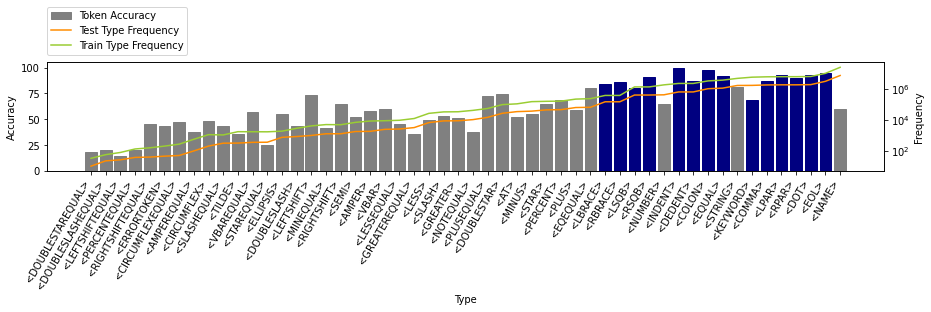
\includegraphics[width=\textwidth]{figures/pycoder_type_discussion_grammar.png}
    \caption{The chart of the token-level code prediction accuracy in token type granularity sorted by the type frequency from small (left) to large (right).}
    \label{fig:type_barplot}
\end{figure*}

% \textbf{Approach.} To answer this research question, we study the difference between following decoding methods. 

% \begin{itemize}
    \item \textbf{Greedy} is a method to select the maximum probable vocabulary to be the next tokens.
    This method assumes that the model already outputs the best probability in every timestep.
    % it generates all possible tokens in the vocabulary list; then, it will choose top B candidates that have the most probability. Those B candidates will move to the next time step, and the process repeats. In the end, there will only be B candidates. The search space is only (10,000)*B.
%     Although selecting only the highest
% probability token is suitable for a specific time step, it
% might be a sub-optimal for a sequence. 
    
    \item \textbf{Beam Search} applies a search algorithm to generate all possible tokens in the vocabulary; then, it selects the top $b$ (i.e., beam size) probable tokens to continue.
    The Beam Search method is one of the most commonly used decoding methods in text generation tasks~\cite{li-etal-2016-deep, wiseman-etal-2017-challenges}.
    % However, Beam Search may not always achieve optimal results, since it does not consider the whole vocabulary, but instead only the top $b$ (i.e., beam size) probable tokens.
    % Nevertheless, Beam Search still performs faster than an exhaustive search.
    
    % ; however, it balances between the performance and the computational time.
    % The method's time complexity is equals to $O(b*V)$ where $V$ is the vocabulary size.
    % It . 
    
    % recommend the most probable $b$ next tokens according to a defined $b$ beam size threshold.

    
    
    
    % by expanding the graph in a limited set called beam~size~($b$).
    % In each timestep, the method generates all possible tokens in the vocabulary; then, it select the top $B$ probability tokens to continue.
      
    
    \item \textbf{Sampling} is a method to randomly select the next token from the actual probability distribution assigned by the model.
    Different from Greedy and Beam search methods which in some cases may recommend only the same probable next tokens at different timesteps, the sampling method may recommend different next tokens at different timesteps (i.e., non-deterministic).
    % We put the sampling method in this study as the baseline for other decoding methods. All of the methods that required sampling are set the seed value to the same number.
    
    % Temperature is used to increase the probability of probable tokens while reducing the one that is not. Usually, the range is 0 < temp ≤ 1. Note that when temp=1, there is no effect.
    \item \textbf{Sampling with Temperature} applies a temperature parameter to shape the probability distribution~\cite{ackley1985learning}, which is different from the original sampling method where the randomness is arbitrary.
    The temperature is used to increase the probability of the most probable next tokens, while decreasing the probability of the others.
    We note that the probability of the least probable next tokens is only decreased, but they are not removed from the recommendation.
    The range of the temperature value is usually at $0 < temp \le 1$, where $temp = 1$ is a normal sampling.

    % Additional to normal sampling which could be arbitrary, sampling with temperature method 
    \item \textbf{Top-K Sampling} aims to truncate the probability distribution by choosing the top-$k$ probable next tokens from the vocabulary, then, re-scale the distribution and perform sampling based on the new distribution.
    This method ensures that the less probable next tokens will not be generated, while only the top-$k$ probable next tokens are only considered during the sampling process.
    
    \item \textbf{Top-P Sampling (Nucleus Sampling)} is similar to the Top-k sampling method where the Top-P sampling method also truncates the probability distribution, but with different criteria. 
    Top-P sampling prunes the distribution by the cumulative probability of the current step $\ge p$~\cite{holtzman2019curious}; then, re-scale and perform sampling.
    Formally, given the probability P, we can define the smallest summation of the probability as $V_p$ in
    \begin{equation}
        \label{eq:top-p}
        \sum_{x\in V_p} P(x|x_{1:i-1}) \ge p
    \end{equation}
    The benefit of this method is that it can dynamically adjust the number of $k$ depending on the certainty of the model.
    If the model is very certain on some tokens, the search space is small, and vice versa.
\end{itemize}
% \textbf{Results.}
% We also compare Beam search from two libraries: CodeXGLUE and HuggingFace.
% For Greedy method, we use Beam search with beam size $b$=1.
% Note that the model we use here is the hard parameter sharing model with task weighing parameter equal to 9:1 (code to type) since it is the best combination from experiments in RQ2 and RQ3.
Since decoding methods are specially designed for generating code predictions as a sequence (i.e., not an individual code token), the rest of this RQ will focus on the line-level predictions only, not the token-level predictions.
% is to handle a search space for a sequence prediction,
% i.e. line-level prediction.
% \kla{???, you can fill}.
% Thus, we will not focus on the impact of decoding methods on the token-level predictions.
% We perform the experiments for this RQ in the line-level prediction since selecting only the highest probability token is suitable for predicting a token\kla{this is the explanation for token-level, not why choosing line-level}, however, it might be a sub-optimal for a sequence.
We note that some decoding methods (i.e., Beam Search and Sampling with a probability shaping function) require parameter settings to be specified.
Thus, we experiment with the following parameters: a beam size ($b$) of $\{3, 5, 10, 16, 50\}$ for Beam Search, a temperature ($temp$) of $\{0.05, 0.1, 0.3, 0.5, 0.7, 0.9\}$ for Sampling with Temperature, a top-k ($k$) of $\{3, 5, 10, 50, 100\}$ for Top-K Sampling, and a top-p ($p$) of $\{0.05,0.1,0.3,0.5,0.7,0.9\}$ for Top-P Sampling.
For the Sampling approaches, we repeat the experiment five (5) times with different seed numbers to ensure the robustness of the results.
Thus, we present the results using the average of the distribution and its standard deviation (SD).
% ; then, the final reported number are the average score and the .
% ......
% \kla{why line level?} 
% We adjust different sizes of  beam size ($b$), top-k ($k$), top-p ($p$) and temperature ($temp$) \kla{why these params?} to our best effort using $b \in \{3, 5, 10, 16, 50\}$, $temp \in \{0.05, 0.1, 0.3, 0.5, 0.7, 0.9\}$,  $k \in \{3, 5, 10, 50, 100\}$, and $p \in \{0.05,0.1,0.3,0.5,0.7,0.9\}$; then, select the best value of each method to compare in this RQ (i.e. $b$=5, $k$=3, $p$=0.1 and $temp$=0.1).
Since Beam Search and Greedy methods are available in both CodeXGLUE and HuggingFace libraries with different implementations, we also evaluate decoding methods using both libraries.
Finally, we experiment with a total of 102 variants of 6 decoding methods, i.e., $\bigl($2*libraries $\times$ (1*Greedy + 5*BeamSearch)$\bigr)$ + $\bigl($5 repeats $\times$ (1*Sampling, 6*Temp, 5*$k$, 6*$p$)$\bigr)$. 

% Thus, we also compare the results to see the impact of decoding methods from the different libraries. 
% We also compare the results between two different libraries: CodeXGLUE and HuggingFace. \kla{why 2 libs?}
% different decoding methods has impact, different library has impact, best is beam search > sampling 



\textbf{Beam Search performs the best, while Sampling performs the worst.}
Table~\ref{tab:rq4} shows that there is a great performance difference of \our~when different decoding methods are used.
For example, Beam Search(CodeXGLUE) generally achieves an exact match of 43.37\%, while Sampling achieves an exact match of 33.80\%, confirming that the decoding methods have a substantial impact on the performance of \our for line-level code completion.
In addition, we find that not only the methods but different libraries with different implementations also produce different results.
In particular, when comparing Beam Search between CodeXGLUE and HuggingFace libraries (see Table~\ref{tab:rq4}), we find that Beam Search from the CodeXGLUE library achieves an exact match of 43.37\% (used by \our), which is greater than that from the HuggingFace library.
This finding suggests that future studies should use Beam Search(CodeXGLUE) for code completion and should report the library used for decoding methods for better reproducibility and replicability details.


% Moreover, the different decoding method implexact matchentations also impact the results.  
% Comparing between two Beam Search implementations (i.e., HuggingFace and CodeXGLUE), the exact match is vary from 41.52\% to 43.37\%.
% \kla{methods / libs - 2 points are mixing - hard to read}
% Table.~\ref{tab:rq4} indicates that considering only HuggingFace library results, there are a significant relative difference around 22.84\% %7.72\% 
% (from 33.80\% to 41.52\%) on the Exact Match and 7.64\% %5.26\% 
% (from 68.72\% to 73.98\%) on the edit similarity between Sampling method and Beam search method respectively.

% \textbf{Our best suggestion is to use Beam search or Greedy search as they are ones of the best performance which also do not require a random seed sampling.}

We find that Sampling is the lowest-performing decoding method, while advanced Sampling (i.e., Sampling with Probability Shaping) tends to perform better, depending on the specified parameter settings.
Through the comprehensive investigation, Top-P sampling performs best when $p$=0.1, and Sampling with Temp performs best when $temp$=0.1.
These optimal parameter settings are domain and context-specific to code completion, which are different from Holtzman~\ea~\cite{holtzman2019curious} who recommend $temp\in[0.5,1]$, $k\in[1,100]$, $p\in[0.9,1)$ for the text generation tasks.
The optimal setting that we achieved for code completion that is different from the recommendations in the NLP text generation field suggests that researchers should experiment with various parameter settings for the problem that tackle, instead of solely relying on suggestions or recommendations from prior work.


% In other words, it indicates that to give the better results, the Sampling method is shaped into the heuristic method similar to Greedy and Beam search that select the high probable tokens.
% As a result, this could imply that unlike in text generation, Beam Search or Greedy method is more suitable to use than the sampling family in the code completion task.

%  for ,  for ,
% that give the comparable results to Beam search and Greedy are out of the common scope.
% A study~\cite{holtzman2019curious} in text generation has mentioned about common parameter values for probability shaping methods which are .
% However, 


% In fact, these best parameters shape the search space by truncate massive probability distributions.
% In our experiments, we found that the best parameter values are out of common scope and are usually the number that truncate massive probability distributions.
% In other words, it indicates that to give the better results, the Sampling method is shaped into the heuristic method similar to Greedy and Beam search that select the high probable tokens.
% As a result, this could imply that unlike in text generation, Beam Search or Greedy method is more suitable to use than the sampling family in the code completion task.
% The supporting reason might be from the fact that words in coding are less flexible than in the text generation that presents many synonym words.

% Therefore, in our setting, although the best method for edit similarity is the Sampling with temperature method with $temp$=0.1,
% % is beam search size 5 in both library.
% our best suggestion is to use Beam search or Greedy search as the difference is small and such methods do not require many parameters tuning or random seed sampling.
% This also consistent with those previous works~\cite{lu2021codexglue, izadi2022codefill} that using Beam search with beam size $b$=5.

\begin{tcolorbox}
\emph{\textbf{RQ4 Summary.} 
\fdfour
% We found that the different decoding methods and libraries have impacts on the quality of predictions, and Sampling methods may not be suitable for code completion task. The best decoding method in our setting is Beam search with beam size $b$=5.
}
\end{tcolorbox}   
 
    \section{Threats to Validity}
\label{sec:threats to validity}

% In this section, we discuss threat to the validity.

% relate to the granularity level of code completion, and the baseline selection.
% Our \our~is trained to work on token-level code completion and can be adapted to line-level code completion.
% Thus, the model is generalized to use in different granularity.

\textbf{Threats to construct validity} relate to the selection of baseline approaches.
In this paper, we select the publicly accessible approach, which could reduce biases and increase the transparency of the comparison of the experimental results. 
Therefore, 
% instead of comparing with nonpublic MTL code completion models~\cite{izadi2022codefill, liu2020self, liu2020multi}, 
we select the competitive state-of-the-art approaches which are publicly available by the authors as the baselines.
We run all the experiments using the replication package and the best hyperparameter settings in their papers.

\textbf{Threats to internal validity} relate to the impact of the hyperparameters on the performance of \our.
To mitigate this threat, we conduct experiments with various hyperparameter settings (see RQ3 and RQ4).
However, we find that \our~is generally robust to the model task weights.
Thus, we suspect that hyperparameters will have a minimal impact on the performance of \our.
Nevertheless, optimizing the hyperparameters of the Transformer model could be expensive and is not the main goal of this paper.
Due to the limited access to premium GPU computing resources, our results serve as a minimum bound, which could be further improved after optimization and with premium GPU access.
Nevertheless, to mitigate this threat, we report the hyperparameter settings in our replication package.

% These hyperarameters haven't be optimized due to the very expensive cost in large search space of Transformer architecture.
% Thus, there might be room for further improvement; nonetheless, the current settings have the considerable performance to compete with the baselines.
% To mitigate this threat, we reports the hyperarameter settings for future replication studies.

\textbf{Threats to external validity} relate to the degree to which our approach can be generalized across other context.
We evaluate our \our~with 50,000 python files from PY150 dataset which is the dataset used in many literature~\cite{lu2021codexglue, kim2021code, izadi2022codefill, li2017code, liu2020self, liu2022unified, wang2020towards}.
We also evaluate the model with the code completion benchmark in CodeXGLUE~\cite{lu2021codexglue}.
However, we limit the scope of this paper to python and have not demonstrated the results to other languages.
Thus, other datasets can be explored in the future work.
   
 
    \section{Conclusion}\label{sec:conclusion}

%1
% Current on-the-fly code completion approaches (e.g. variants of GPT-2 model) consume sequences of source code as inputs to generate the next source code tokens. 
% Such training objective do not need the completeness of source code, however; it does not consider syntactic information.
% To include syntactic information, many research studies leverage the use of ASTs information.
% While predicting the AST nodes may help to ensure the syntactically correct predicted code, the approaches require the complete and syntactically correct code to extract ASTs to be the inputs. 

% ASTs information is hard to be correctly retrieve, therefore we bring forward standard type information which is also represent syntactical structure and easier to retrieve. With \gls{mtl} training technique, we propose TypeComp, the generative type-aware transformers for code completion. We intensively train and test the model on different training techniques and weighing. We also experiment on the variety of decoding methods. In the end, not only we evaluate our best model to many replication of state-of-the-art code completion, but we also send the results to evaluate on CodeXGLUE Benchmark. The results show that our model surpass all baselines in both token-level predictions and line-level predictions.

%2
% Code completion is an essential feature to help improve developers' performance; however, there are limitations in the previous approach.
% The GPT-variants code completion approach does not need the completeness of source code (i.e. on-the-fly); however, it does not consider syntactic information.
% To include syntactic information (i.e. syntactic-aware), many research studies leverage the use of ASTs information which require the complete and syntactically correct source code available before it can be extracted.
% These yield to the limitation that current approaches are either on-the-fly or syntactic-aware but not both.

% To address these limitations, we propose \our~to leverage token types, a kind of lightweight syntactic information, with a multi-task training strategy that  learning on the supporting task of predicting token types during the training phase.
% We intensively train and test our \our~on different multi-task training techniques, task weighing parameters, and decoding methods to find the best suitable architecture.

% In the evaluation, \our~surpasses all four state-of-the-art approaches which includes both AST-based and non-AST based models.
% Specifically, relative to the second best models, our models achieves with an improvement in accuracy of 1.89\% (from 75.69\% to 77.12\%) in token-level prediction and an improvement in exact match of 8.34\% (from 40.03\% to 43.37\%) in line-level prediction.
% Additionally, \our~also receives the first place on code completion task in CodeXGLUE benchmark.
% The results highlight that the token type syntactic information can be beneficial in code completion.
% Thus, \our~could potentially be beneficial to developers on suggesting the code tokens or lines which could help improve developers' performance by reducing effort on coding.

In this work, we propose \our~to leverage token types, a kind of lightweight syntactic information, with a multi-task training strategy that learning on the supporting task of predicting token types during the training phase.
We intensively train and test our \our~on different multi-task training techniques, task weighing parameters, and decoding methods to find the best suitable architecture.
Our study underline the following conclusion:
\begin{itemize}
    \item \our~surpasses all the state-of-the-art models in our setting and also receives the first place in CodeXGLUE’s python code completion benchmark. The results indicate that the token type syntactic information can be beneficial in code completion.
    \item In our setting, MTL: Hard Parameter Sharing -- PyCoder-Hard with task's weight (Type:Code) 1:9 and Beam Search performs the best. 
    \item  Our study highlights the importance of investigating various choices of setting (e.g., multi-task training strategies, parameter setting) instead of solely relying on suggestions from prior work.
\end{itemize}
Our \our~has extended the feature of on-the-fly code completion with lightweight syntactic-aware information.
However, we acknowledge that there is still a space to develop the fully syntactically correct code completion model with on-the-fly feature.
We leave this exploration for the future research study.
   

   \bibliography{mybibfile}   



\end{document}
